\chapter{Introduction to the Ubiquitin 26S Proteasome System}

Adapted in part from: R.S. Marshall*, D.C. Gemperline*, and R.D. Vierstra (2015). Purification of 26S proteasomes and their sub-complexes from plants. \textit{Methods Mol. Biol.} DOI: 10.1007/978-1-4939-6533-5 \\

\noindent
*These authors contributed equally to the \textit{Methods Mol. Biol.} work. \\

\noindent
This chapter has expanded sections on the proteasomes role in plant biology, proteasome assembly, and proteasome isotypes. \\

\section{The Ubiquitin 26S Proteasome System (UPS)}
	Selective proteolysis in plants plays a critical role in both regulating growth and development, and maintaining cellular homeostasis \citep{nelson14, smalle04, vierstra93, vierstra09}.  One of the principle pathways for protein degradation in plants and other eukaryotes is the ubiquitin-26S proteasome system (UPS), which involves the attachment of polyubiquitin chains to target proteins followed by their recognition and degradation by the 26S proteasome, an exquisitely designed proteolytic machine \citep{bhattacharyya14, finley09, vierstra09}.  The UPS is highly conserved across all eukaryotes; it was first elucidated by elegant work in rabbit reticulocyte lysates \citep{ciechanover80, ciechanover80-frAQB, etlinger77, hershko80, wilkinson80}, and was subsequently identified in other animals, yeast and plants \citep{ciechanover84, finley84, finley87, glotzer91, hochstrasser91, shanklin87}.  Ubiquitin conjugation to target proteins is accomplished through a highly polymorphic, ATP-dependent cascade involving the sequential action of three enzyme classes, termed the E1 ubiquitin-activating enzymes, E2 ubiquitin-conjugating enzymes, and E3 ubiquitin-protein ligases \citep{berndsen14, smalle04, vierstra09} (Figure \ref{fig:upscycle}).  Selectivity in ubiquitylation is typically driven by the E3 family, which has dramatically expanded during plant evolution to include well over a thousand variants in Arabidopsis and other plant species \citep{hua13, hua11}. Indeed 6\% of the Arabidopsis proteome is devoted to UPS \citep{smalle04}. 

\begin{sidewaysfigure}[p]
	\centering
	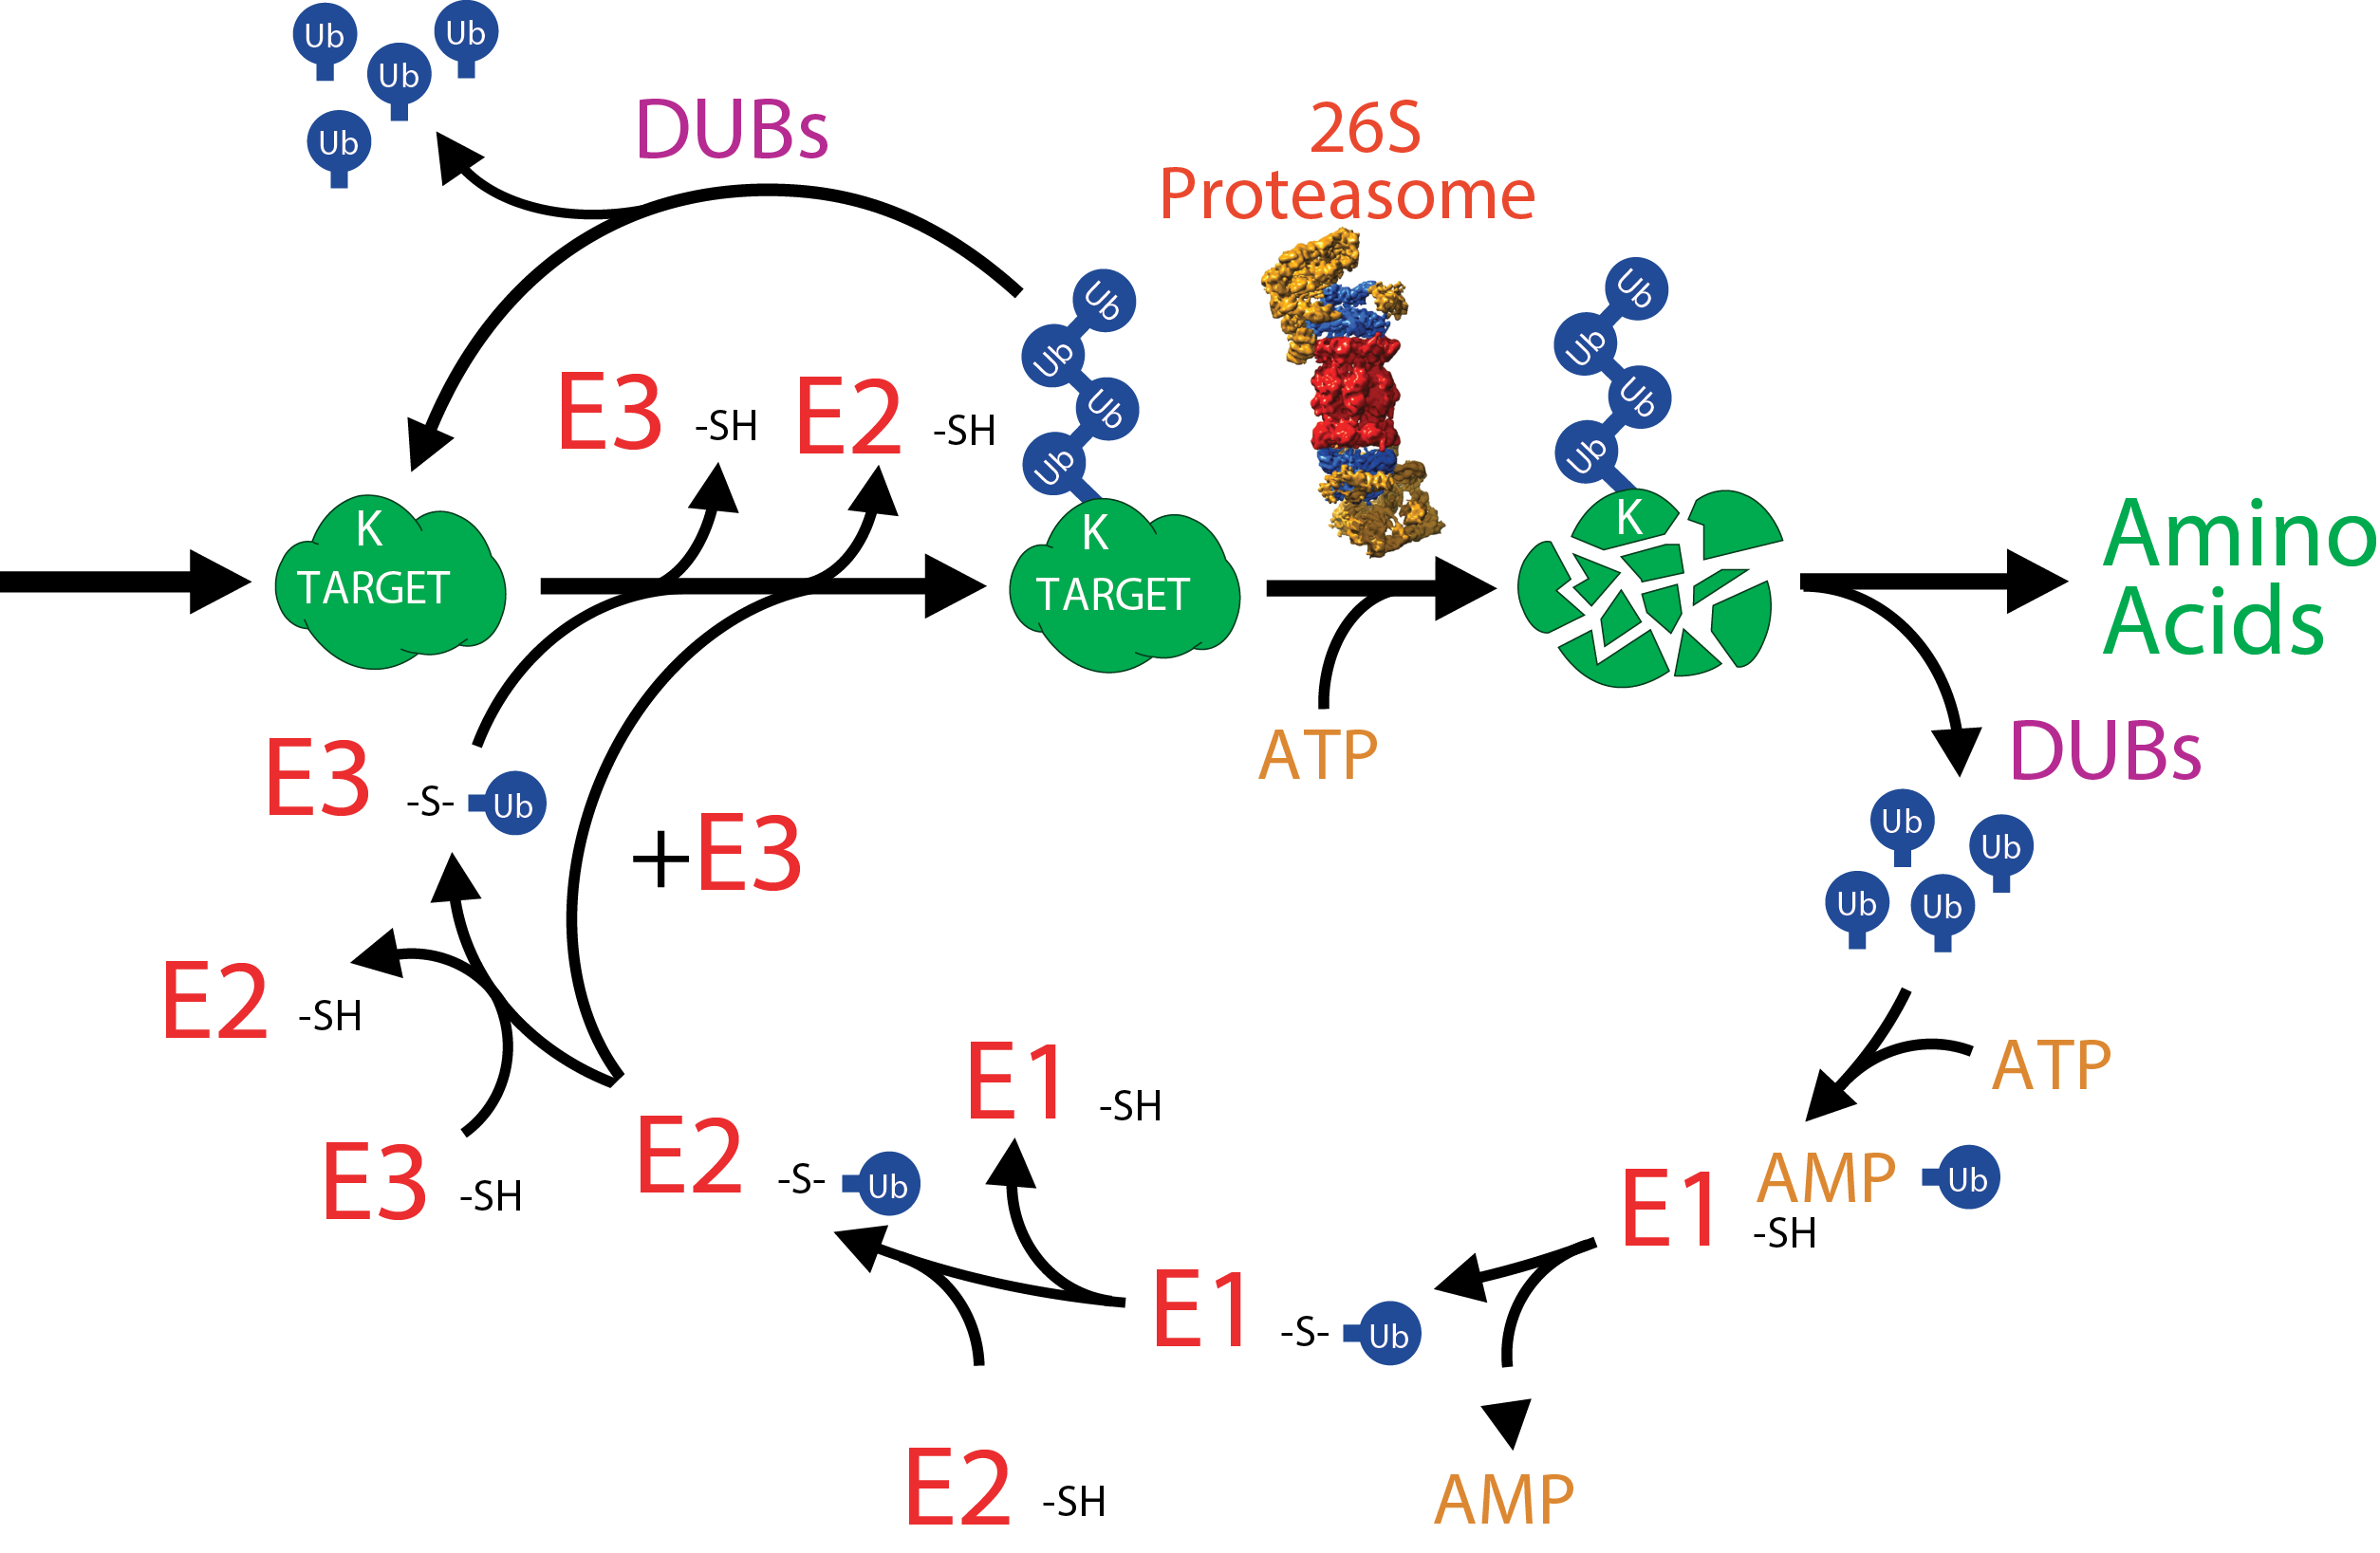
\includegraphics[width=\columnwidth]{intro/upscycle.png}
	\mycaption{A schematic representation of the E1 activating, E2 conjugating, and E3 ligase enzymatic cascade for the covalent attachment of the small polypeptide Ubiquitin to target protein lysines}{
Once a protein becomes polyubiquitylated it is efficiently recognized by the 26S proteasome. The rate of addition of ubquitins, and the rate of removal by de-ubiquitylating enzymes (DUBs) determines the final equilibrium of degradation.}
	\label{fig:upscycle}
\end{sidewaysfigure}

	The UPS helps regulate plant growth and development by regulating several key proteins including those involved in morphogenesis, light sensing, and the circadian clock (reviewed in \citep{vierstra09}. Some examples include E3 enzymes such as BIG BROTHER that controls organ size \citep{disch06}, F-BOX-LIKE 17 that helps regulate spermatogenesis \citep{kim08}, and UNUSUAL FLORAL ORGANS which regulates floral development \citep{samach99}. The UPS also helps regulate plants response to light by degrading phytochrome A \citep{clough97, shanklin87}, a key photoreceptor in plants. An E3 ligase ZTL also aides in removing TOC1 involved in circadian clock regulation \citep{más03}. 

	Additionally, the UPS also aides in the regulation of key plant hormonal responses including auxin, abscisic acid, jasmonic acid (JA), giberellins (GA), and ethylene. (reviewed in \citep{santner10}). Key hormone response factors are degraded by a variety of E3 complexes including TIR1 involved in auxin regulation \citep{dharmasiri05}, COI1, involved JA sensing \citep{katsir08}, and GID1 involved in GA responses \citep{murase08}. An elegant mechanism requires the direct binding of these key hormones either to their respective E3 complexes, or key proteins associated with these E3's to promote the efficient ubiquitylation and subsequent degradation of their hormone response factors \citep{shabek14}. 

	The UPS is both co-opted and inhibited by several plant pathogens that helps aide in their virulence. The plant pathogen \textit{Ralstonia solanacearum} encodes a suite of E3 enzymes that co-opt host machinery to evade plant defense responses \citep{angot06}. Additionally, \textit{Pseudomonas syringae}, a tomato pathogen, secretes a small molecule that irreversibly binds the host 26S proteasome to prevent plants from actively ubiquitylating and degrading key virulence factors \citep{schellenberg10}. 

	Self-incompatibility is a key process in plants that encourages plants to outcross helping aide in plant evolution and diversity by preventing inbreeding \citep{zhang09}. Upon incompatible pollination an E3 enzyme ARC1 helps to ubiquitylate compatibility factors in the pistil leading to self-pollen rejection \citep{stone03}. In another example S-RNase, which acts to degrade the RNA from self-pollen tubes preventing their growth, is actively ubiquitylated via SLF and SSK1 \citep{mcclure04, zhao10}. From these and other analyses it is clear that the UPS either directly, or indirectly, regulates many aspects of plant growth and development including hormone responses, pathogen interactions, and self-incompatibility. Therefore, a fundamental understanding of the UPS system in plants has important agricultural impacts.     

\section{The 26S Proteasome}
	The 26S proteasome is the central enzymatic effector of the UPS, and is a 2.5 MDa particle located in the cytosol and nucleus of eukaryotic cells.  It is composed of two functionally distinct sub-complexes; the 20S core protease (CP) that houses the proteolytic active sites, and the 19S regulatory particle (RP) that recognizes appropriate substrates (Figure \ref{fig:proteasome} A and B; \citep{bhattacharyya14, finley09, lander12, lasker12, unverdorben14}).

\begin{figure}[p]
	\centering
	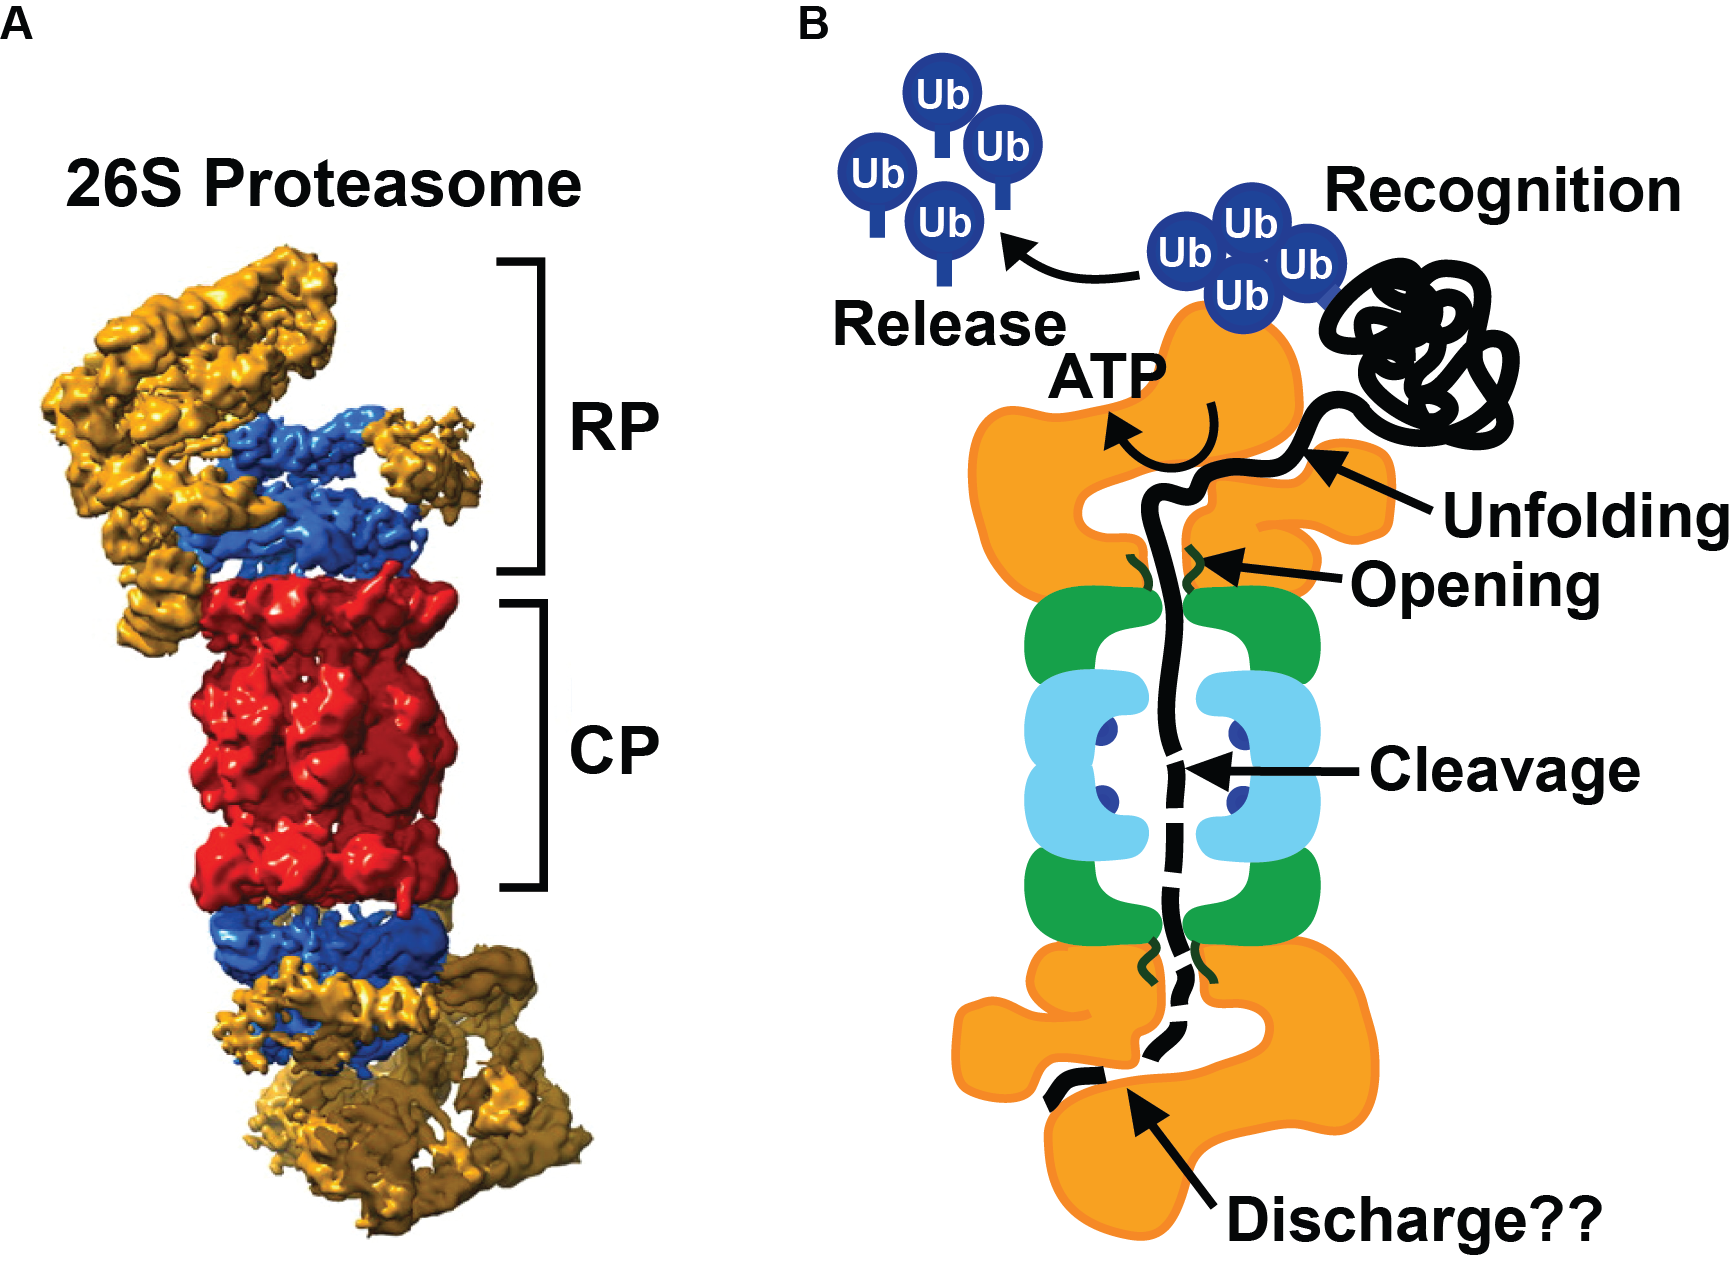
\includegraphics[width=\columnwidth]{intro/proteasome.png}
	\mycaption{The 26S proteasome is made up of two functionally distinct sub-particles.}
	{ \textbf{(A)} The Core Protease (CP) is shown in red, while the Regulatory Particle (RP) is shown in blue for the RPT subunits, and in gold for the RPN subunits (adapted from \citep{lasker12}. \textbf{(B)} Schematic representation of CP and RP functions. The RP is responsible for recognizing and unfolding polyubiquitylated substrates into a central axial chamber upon which the unfolded polypeptide is cleaved by the CP. The RP is also responsible for releasing the ubiquitin so that it can be recycled for re-use through the de-ubiquitylating activity of the metalloprotease RP subunit RPN11. }
	\label{fig:proteasome}
\end{figure}

The CP has a barrel shape generated by four stacked hetero-heptameric rings, which contain seven $\alpha$-subunits or seven $\beta$-subunits (termed PAA-PAG and PBA-PBG, respectively, in \textit{Arabidopsis}) in an $\alpha$1-7/$\beta$1-7/$\beta$1-7/$\alpha$1-7 configuration (Figure \ref{fig:cpdetails} A (side view- stacked rings), C (top view- $\alpha$-subunits) and D (top view- $\beta$-subunits).

\begin{FPfigure}[Figure \ref{fig:cpdetails} \textit{caption follows on next page}]
	\centering
	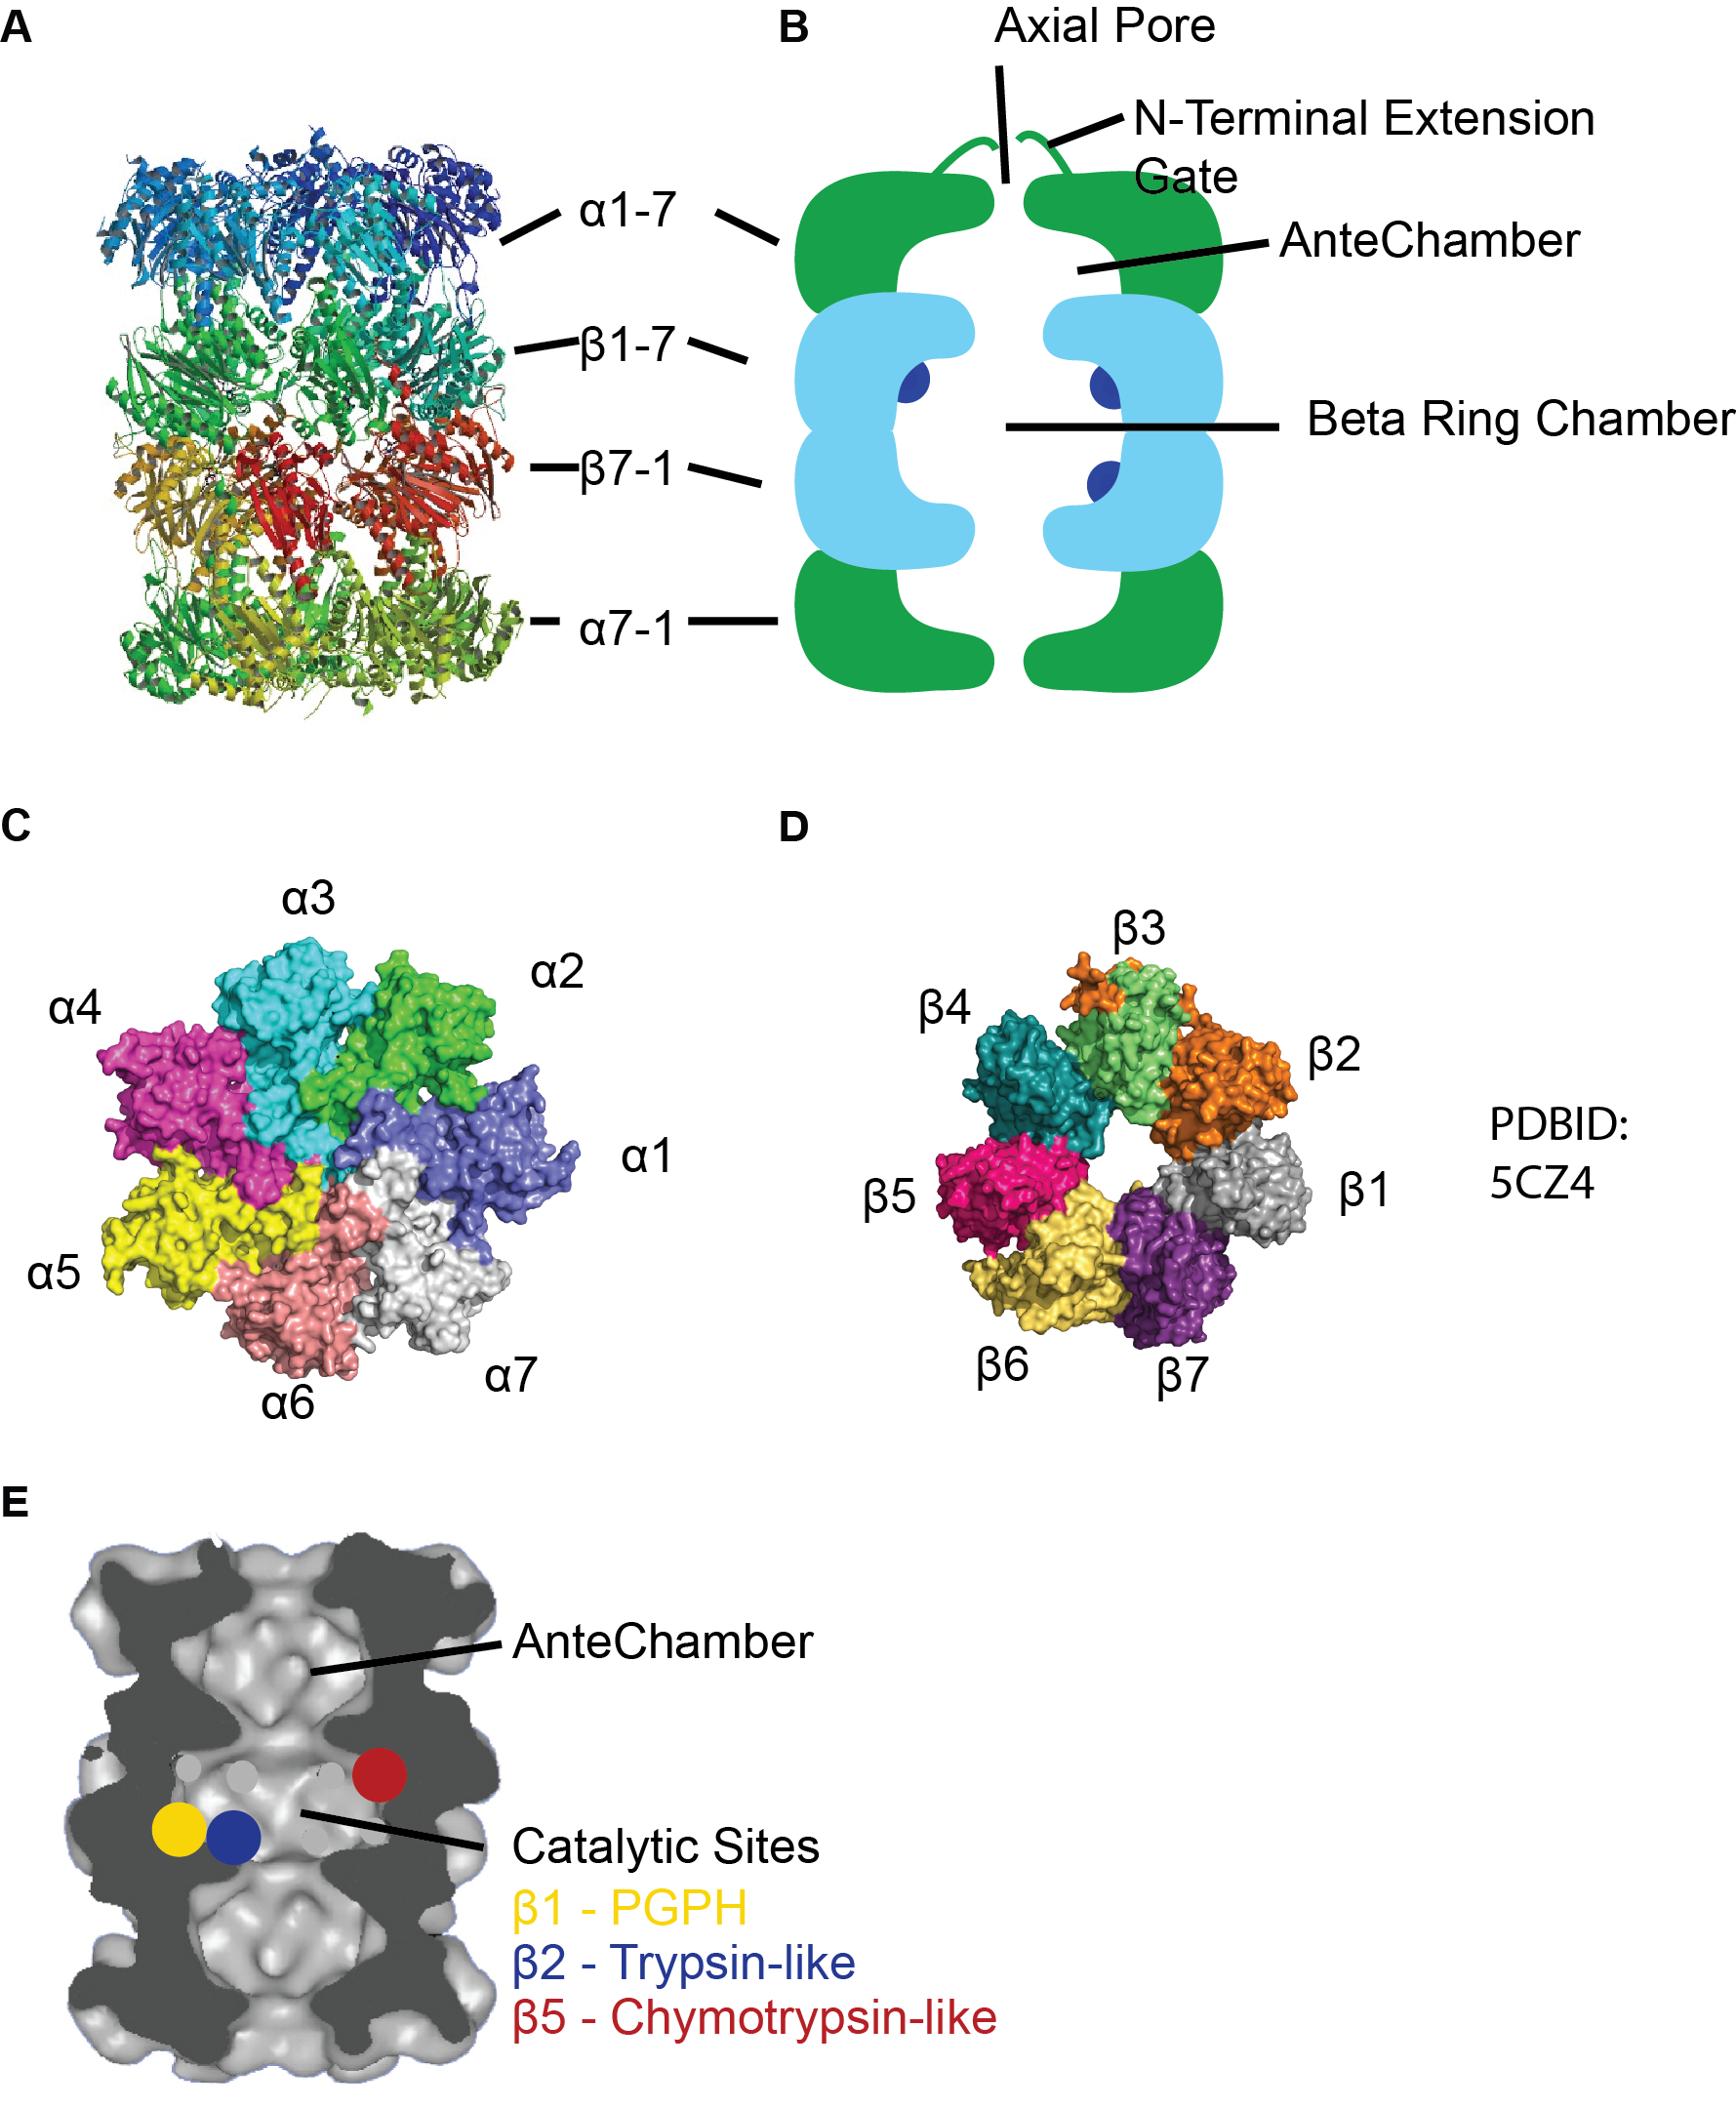
\includegraphics[width=\columnwidth]{intro/cpdetails.png}
	\mycaption{The 20S Core Protease (CP)}
	{\textbf{(A)} An x-ray crystallographic structure of the 20S CP shows its barrel-like structure. The structure is composed of four stacked hetero-heptameric rings in an $\alpha$1-7, $\beta$1-7, $\beta$1-7, $\alpha$,1-7 configuration. \textbf{(B)} This stacked configuration generates an interior structure amenable to cleaving unfolded polypeptides that enter through the axial pore. N-terminal extensions present in $\alpha$-subunits gate the entry to the antechamber. The antechamber helps maintain the polypeptide in an unfolded state, and the $\beta$-ring chamber houses the catalytic activities of the CP. \textbf{(C)} Top-down view of the CP showing the $\alpha$-subunit configuration (PDB ID 5CZ4) visualized in PyMOL \citep{PyMOL}. \textbf{(D)} Top-down view of the CP showing the $\beta$-subunit configuration (PDB ID 5CZ4) visualized in PyMOL. \textbf{(E)} Catalytic activities of the 20S proteasome are conferred by the $\beta$1 (peptidylglutamyl-peptide hydrolyzing (PGPH)), $\beta$2 (Trypsin-like), and $\beta$5 (Chymotrypsin-like) subunits. A slice through the middle of a model of the 20S proteasome (adapted from \citep{kisselev12}) shows the location and type of the three catalytic activities of the 20S proteasome. While this is a half-structure, each barrel actually houses 6 catalytically active locations, with three different catalytic activities.}
	\label{fig:cpdetails}
\end{FPfigure}

Upon assembly, a central chamber is formed at the $\beta$-ring interface that houses six peptidase catalytic sites provided by the $\beta$1 (PBA), $\beta$2 (PBB), and $\beta$5 (PBE) subunits \citep{arendt97, heinemeyer97} (Figure \ref{fig:cpdetails} B and E).  The active sites involve a catalytic triad, one residue of which is an N-terminal threonine that becomes exposed during CP assembly.  Collectively these peptidases can cleave a broad range of protein sequences with peptidylglutamyl-peptide hydrolyzing (PGPH) ($\beta$1), trypsin-like ($\beta$2), and chymotryptic-like ($\beta$5) activities \citep{arendt97, groll99} (Figure \ref{fig:cpdetails} E).  The $\alpha$-rings create two antechambers with narrow opposing axial pores that are gated by extensions at the N-terminus of several subunits (Figure \ref{fig:cpdetails} B) \citep{groll00, ruschak10}.  Through this distinctive architecture, the CP acts as a self-compartmentalized protease that will only degrade polypeptides that are deliberately recognized, unfolded, and imported into the $\beta$-ring chamber.



	
	The CP is capped at one or both ends by the RP, which sits on top of the axial pores.  The RP provides activities for recognition of ubiquitylated proteins, substrate unfolding and import, and release of the ubiquitin moieties before substrate degradation (Figure \ref{fig:proteasome}).  Its binding to the CP is stabilized by ATP, which is thus a necessary ingredient for purifying intact 26S proteasomes \citep{smith05}. The RP itself consists of two sub-complexes; the base, which contains a hexameric ring of AAA-ATPases (RPT1-6) plus two non-ATPase subunits, RPN1 and RPN2; and the lid, which is composed of an additional 11 non-ATPase subunits, RPN3, RPN5-13 and DSS1/SEM1 (Figure \ref{fig:proteasome}; \citep{bhattacharyya14, book10, finley09, glickman98-c8Wsa, russell13}.  This lid/base demarcation was first revealed by the absence of lid subunits in proteasomes isolated from a \textit{Δrpn10} yeast deletion strain, and it was hence thought that RPN10 helps enforce binding of the lid to the base \citep{glickman98}.  However, more recent structural studies have demonstrated that RPN10 has a more indirect stabilizing role via its interaction with RPN9 \citep{lander12}.  The ring of RPT subunits in the base promotes substrate unfolding through ATP hydrolysis, and gates the $\alpha$-ring axial pores through repositioning of the CP $\alpha$-subunit extensions \citep{köhler01, rabl08, smith05}.  The N-terminal regions from proximal RPT pairs intertwine to create three spokes onto which most RPN subunits are scaffolded (Figure \ref{fig:rpdetails} A; \citep{beck12}).

\begin{FPfigure}[Figure \ref{fig:rpdetails} \textit{caption follows on next page}]
	\centering
	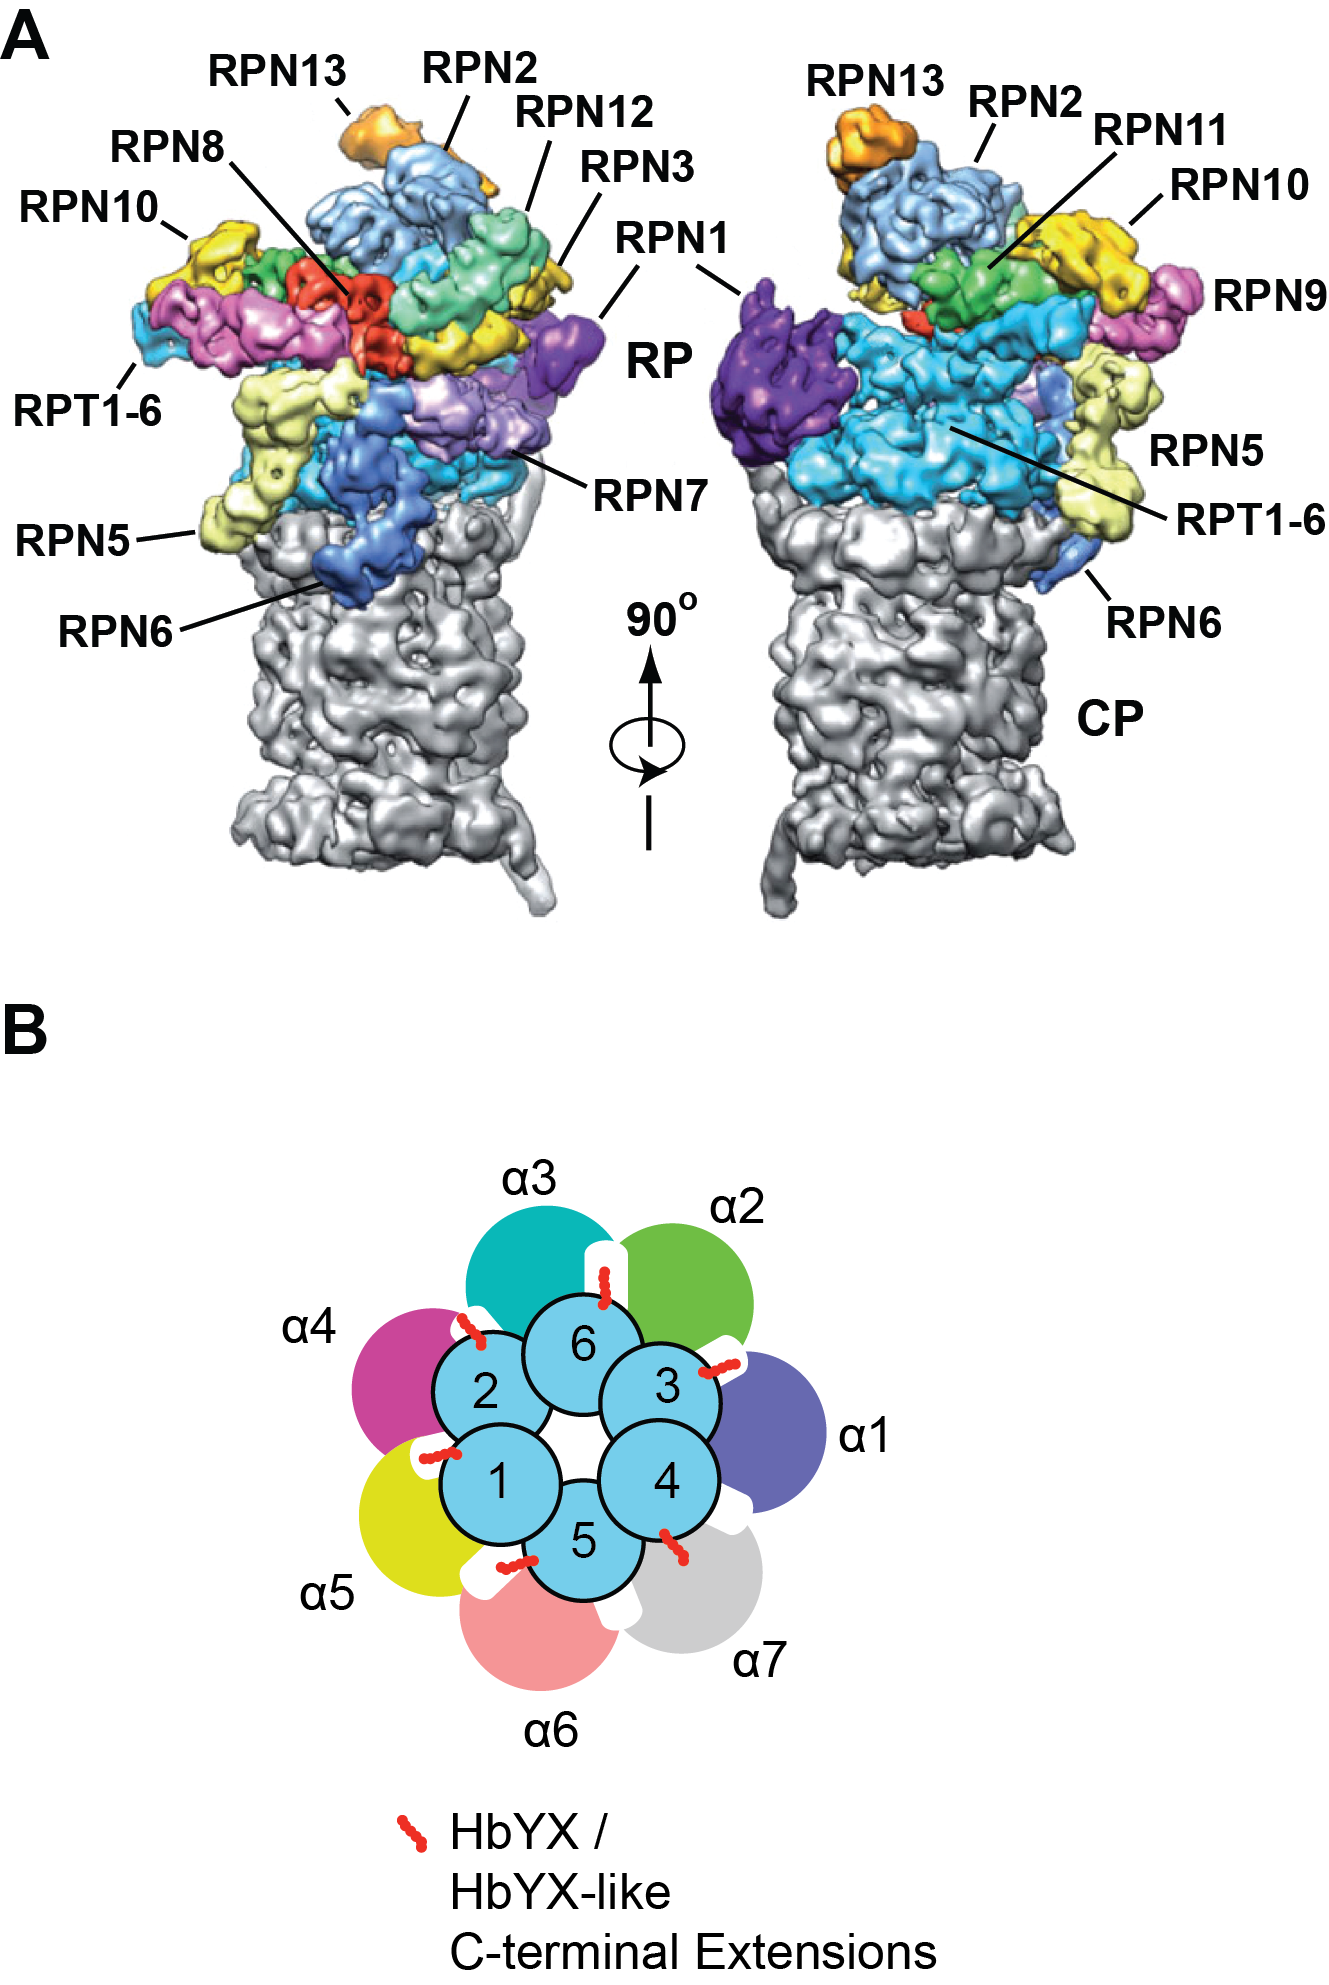
\includegraphics[width=\columnwidth]{intro/rpdetails.png}
	\mycaption{Cryo EM Structure of the 19S Regulatory Particle (RP)}
	{\textbf{(A)} The RP structure as solved by Cryo-EM is shown (modified from \citep{lander12}). In the center in blue are the RPT1-6 subunits, while the RPN subunits are individually labeled. A 90-degree rotation is shown so that the other side of the RP can be visualized. \textbf{(B)} A schematic representation of how the RP subunit C-termini containing HbYX and HbYX-like motifs intercalate between the $\alpha$-subunits (adapted from \citep{sokolova15}). Gaps between each $\alpha$-subunit are shown, and the HbYX motifs are shown as red strands.}
	\label{fig:rpdetails}
\end{FPfigure}

Several RPT subunits harbor C-terminal \textit{Hydrophobic-Tyrosine-Any} amino acid (HbYX) motifs important for their binding to the $\alpha$-subunits in the CP. These C-terminal HbYX and HbYX-like extensions typically intercalate between adjacent $\alpha$-subunits (Figure \ref{fig:rpdetails} B). The RPN6 subunit acts as a molecular clamp to tether the RP onto the CP (Figure \ref{fig:rpdetails} A) \citep{pathare12}. 
	 
\section{Proteasome Purification Strategies}
	Even before the realization that the 26S proteasome is a protease, sub-particles of the complexes were described.  The first reports of proteasomes used avian erythroblast preparations enriched by differential ultracentrifugation followed by fractionation through a sucrose gradient \citep{schmid84}.  These 20S fractions isolated in the absence of added ATP were found to inhibit mRNA translation in a cell-free system, leading to early proposals that the identified complex repressed gene expression through a cryptic ribonuclease activity.  This lead to the particle initially being named the ``prosome'' \citep{kremp86, schmid84}.  Subsequent analyses of these preparations by SDS-PAGE and electron microscopy revealed the signature ladder of $\alpha$- and $\beta$-subunits at 20-35 kDa, as well as their barrel-like architecture (Figure \ref{fig:emstructure} A and B; \citep{baumeister88, kremp86, schmid84}).

\begin{figure}[p]
	\centering
	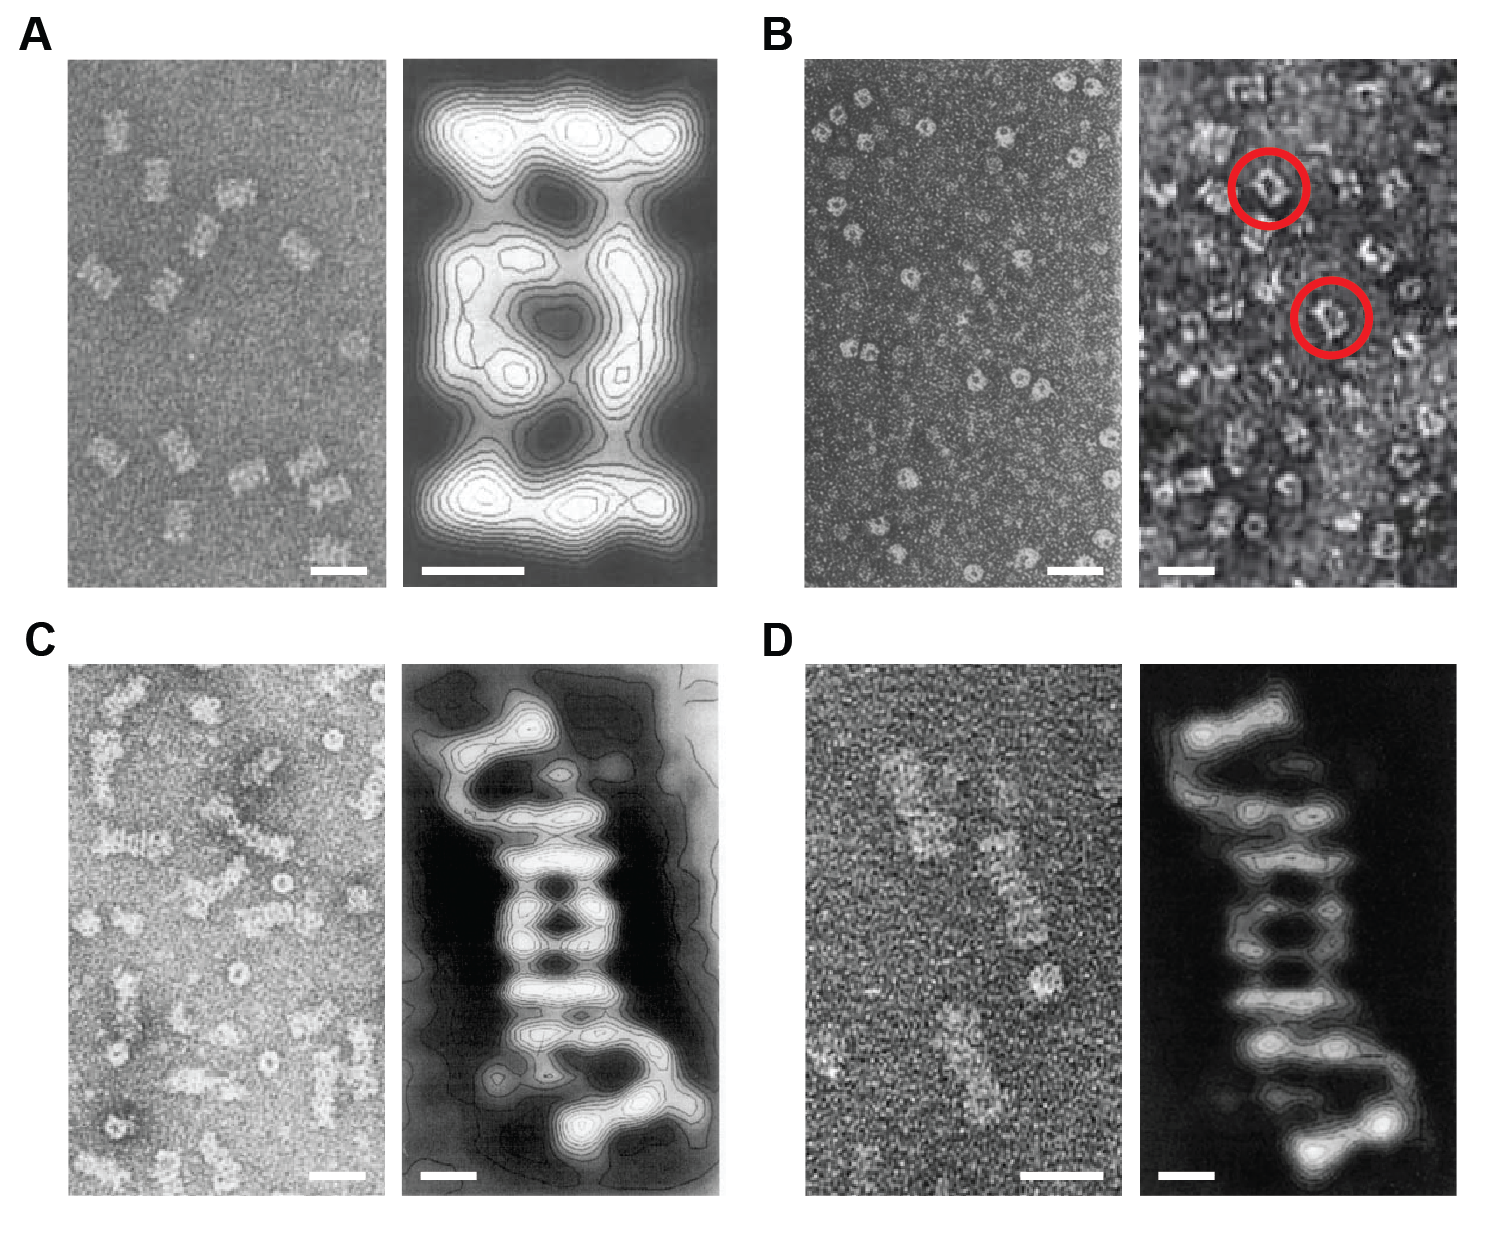
\includegraphics[width=\columnwidth]{intro/emstructure.png}
	\mycaption{Electron microscopy images of 20S and 26S proteasomes from mammals and plants}
	{\textbf{(A)} Images of 20S proteasomes purified from rat skeletal muscle. On the left is an electron micrograph of the 20S particles negatively stained with sodium phosphotungstate, while on the right is a close-up image with overlaid contour plots generated by correlation averaging of approximately 300 individual images negatively stained with ammonium molybdate. \textbf{(B)} Images of the first 20S proteasomes purified from different plant species. On the left are proteasomes isolated from tobacco leaves, while on the right are proteasomes from potato tubers, both negatively stained with uranyl acetate. The typical barrel-shaped structures are indicated with red circles. \textbf{(C)} Images of 26S proteasomes purified from rat liver. On the left is an electron micrograph of the 26S particles negatively stained with uranyl acetate, while on the right is a close-up image with overlaid contour plots generated by correlation averaging of 215 individual images. \textbf{(D)} Images of 26S proteasomes purified from spinach leaves.  On the left is an electron micrograph of the 26S particles negatively stained with uranyl acetate, while on the right is a close-up image with overlaid contour plots generated by correlation averaging of 450 individual images. In all cases, scale bars represent 25 nm for the electron micrograph images and 5 nm for close-up images generated by averaging. The images were modified from references \citep{baumeister88, fujinami94, kremp86, schliephacke91, yoshimura93}.}
	\label{fig:emstructure}
\end{figure}

Purification of the 20S fraction from HeLa cells followed by SDS-PAGE also gave rise to this stereotypical protein banding pattern and shape \citep{schmid84}, and this was followed shortly thereafter by the first description of plant prosomes, purified from tobacco leaf extracts using similar sedimentation protocols in ATP-free buffers \citep{kremp86}.  In these later cases, the purified preparations had strong peptidase activity but little to no RNase activity, thus leading to the conclusion that the CP is actually a protease.  Once its true function in protein turnover was confirmed, the moniker for the particle was changed to ``proteasome'' \citep{arrigo88}.  
	
	Subsequently, the 20S particle was purified from other plant tissues, including dry pea seeds, potato tubers, mung bean seedlings, and leaves from both spinach and wheat \citep{murray97, ozaki92, schliephacke91, skoda92}.  These purifications were typically performed using sequential anion exchange and size-exclusion chromatography steps in the absence of ATP, hence only the CP was isolated.  Their remarkable similarity in protein composition and structure, as observed by SDS-PAGE and electron microscopy, respectively, coupled with the fact that several of the plant subunits cross-reacted with antibodies against their yeast, human, rat and \textit{Xenopus} counterparts, strongly implied that the CP was conserved and widely distributed among eukaryotes \citep{schliephacke91}.
	
The complete 26S proteasome (i.e. the CP capped at one or both ends by the RP) was subsequently discovered by the purification of ubiquitin conjugate-degrading activity from rabbit reticulocytes \citep{hough86}.  While it had been well established that major catabolic processes in animal cells involved the ATP-dependent proteolysis of selective substrates \citep{etlinger77}, the enzyme(s) responsible for this activity had yet to be identified.  Taking advantage of the new ability to synthesize ubiquitylated substrates such as 125I-labelled ubiquitin-lysozyme conjugates \citep{hough86-1xVPf}, a protocol was developed to purify the responsible ATP-dependent protease.  Through a series of anion exchange and size exclusion chromatography steps followed by glycerol gradient sedimentation, all of which were performed in ATP-containing buffers, the responsible activity was isolated \citep{hough86, hough87}. The active enzyme turned out to be the 20S proteasome (i.e. the CP) along with a number of additional polypeptides, which together formed a 26S particle, thus providing the first direct link between ubiquitylation and a protease \citep{ganoth88, hough87, waxman87}.  SDS-PAGE analysis of these preparations identified a host of new polypeptides in the 35-100 kDa range in addition to the known CP subunits, which were later shown to comprise a second stable complex, the RP.  Shortly thereafter, the RP was demonstrated to have ATPase activities attributable to the RPT subunits, which help in substrate unfolding and maintaining CP-RP association \citep{armon90}.  Electron microscopic images of the full 26S particle then revealed its diagnostic quaternary structure in which the CP is capped by one or two RPs that sit over the axial pores for substrate entry (Figure \ref{fig:emstructure} C; \citep{peters91, yoshimura93}).

The existence of a similar 26S proteasome in plants was initially implied by the detection of an ATP-dependent activity in oat and wheat germ extracts capable of degrading ubiquitylated proteins \citep{hatfield89, vierstra88}.  This was followed some years later by the first isolation of a complete plant 26S proteasome holocomplex from spinach leaves \citep{fujinami94}.  As with the mammalian forms, purification was achieved by anion exchange and size exclusion chromatography, followed by glycerol gradient centrifugation, all in the presence of ATP to stabilize the CP-RP association.  These spinach preparations were, like their rabbit reticulocyte counterparts, able to rapidly degrade ubiquitylated substrates in an ATP-dependent manner, and further analysis by native-PAGE, SDS-PAGE and electron microscopy revealed the complete subunit composition and “caterpillar-like” structure of the plant particle (Figure \ref{fig:emstructure} D; \citep{fujinami94}).  Similar purifications were successful using rice suspension culture cells and garlic cloves \citep{malik04, yanagawa99}, which were accompanied by the first demonstrations that proteasome inhibitors designed for their mammalian counterparts were effective with the plant particles, suggesting very similar enzymatic mechanisms \citep{ozaki92, woffenden98}.  

Despite its prevalence as a genetic model, purification of the 26S proteasome from the flowering plant \textit{Arabidopsis thaliana} was not reported until several years after other plant species \citep{yang04}.  First protocols involved differential PEG precipitation followed by anion exchange and size exclusion chromatography, with the latter exploiting the large size of the holoprotease.  More recently, an improved one-step affinity method was developed \citep{book10}, based on the strategies that had been successfully employed in yeast \citep{leggett05}.  Here, epitope-tagged proteasomes were generated by genetically replacing the subunit PAG1 with a variant bearing a C-terminal FLAG tag; this tagged particle could then be purified with appropriate affinity matrices, and released in non-denaturing conditions with FLAG peptide.  This approach enables rapid and robust purification of the whole 26S proteasome complex when performed in the presence of ATP, or enables purification of the CP sub-particle when performed in the absence of ATP \citep{book10}. This affinity method has considerable advantages compared to previous, conventional chromatographic approaches \citep{yang04} as it is both faster, more reliable and produces higher yields per gram of tissue (\textasciitilde{}6 µg/g). This milder more rapid technique also prevents breakdown of some subunits, in particular RPN10, which is sensitive to post-homogenization proteolysis \citep{yang04}.  One caveat is that the epitope tag, given its exposed position and flexible structure, might be sensitive to proteolytic cleavage following tissue homogenization.  For the PAG1-FLAG protocol, chymostatin was found to effectively block the interfering protease \citep{book10}. An example of such preparations analyzed by SDS-PAGE followed by immunoblotting with antibodies against several proteasome subunits, is shown in Figure \ref{fig:pag1flagap}.

\begin{figure}[p]
	\centering
	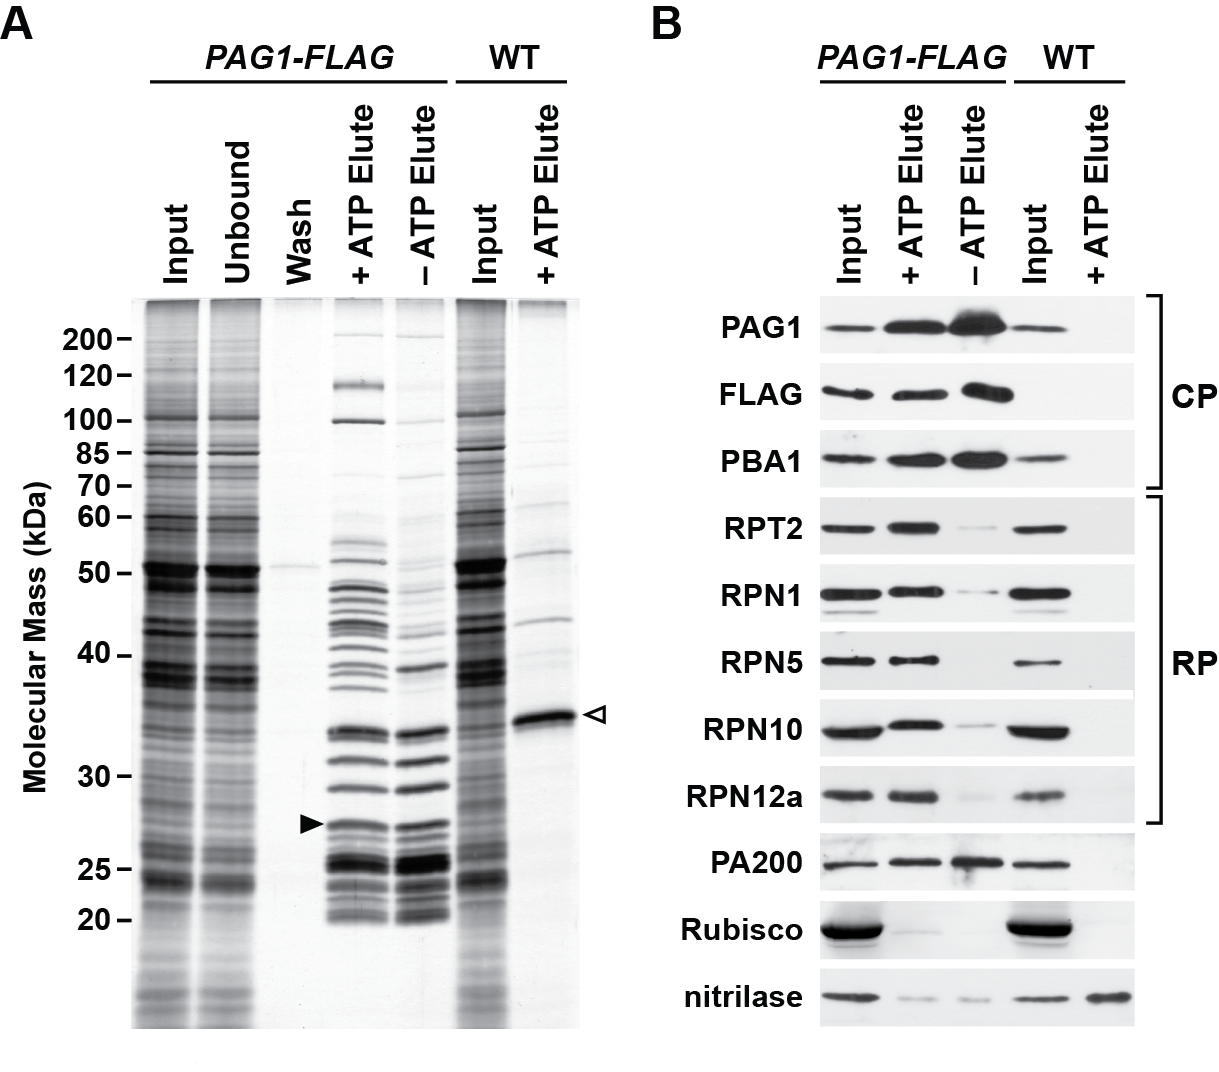
\includegraphics[width=\columnwidth]{intro/pag1flagap.png}
	\mycaption{Affinity purification of 26S proteasomes from \textit{PAG1::PAG1-FLAG pag1-1} plants}
	{\citep{book10} \textbf{(A)} SDS-PAGE analysis of proteins obtained at each affinity purification step.  Total protein extracts from 10 day old wild-type (WT) and \textit{PAG1::PAG1-FLAG pag1-1} plants were incubated with anti-FLAG affinity resin, washed, and competitively eluted with the FLAG peptide. The procedure was performed in the presence or absence of ATP, and the input, unbound, washed and eluted fractions were subjected to SDS-PAGE and the gel stained for protein with silver.  The black arrowhead indicates the PAG1-FLAG protein, while the open arrowhead identifies nitrilase, which is non-specifically enriched during the purification. \textbf{(B)} Immunoblot detection of various 26S proteasome subunits in the affinity-purified preparations shown in A. Subunits tested include the CP subunits PAG1 and PBA1, the RP subunits RPT2, RPN1, RPN5, RPN10 and RPN12a, and the alternate capping particle PA200.  Other proteins tested include the Rubisco small subunit and nitrilase. This figure was modified from reference \citep{book10}.}
	\label{fig:pag1flagap}
\end{figure}

\section{26S Proteasome Substrate Processing}
A variety of proteins help the 26S proteasome process ubiquitylated substrates. Some include key constituents of the complex itself, such as RPN11, which is a metalloprotease that uses a zinc-coordinated active site to release the ubiquitin moieties isopeptide-linked to substrates \citep{verma02, worden14}.  Through RPN11 and other loosely associated deubiquitylating enzymes such as UBP6/USP14 \citep{hanna06, sakata11}, bound ubiquitins are actively recycled. 
Substrate selection by the 26S proteasome is dictated by several ubiquitin receptors intrinsic to the RP lid, including RPN1, RPN10, RPN13, and DSS1/SEM1 \citep{elsasser02, fatimababy10, finley09, lin11, paraskevopoulos14, sakata12, shi16, van96}.  RPN10 binds ubiquitin via defined ubiquitin-interacting motifs (UIMs), of which yeast, human and \textit{Arabidopsis} RPN10 contain 1, 2 and 3 in tandem, respectively \citep{fatimababy10, finley09, fu98, lin11, van96}.  By contrast, RPN13 binds ubiquitin via a pleckstrin-like receptor for ubiquitin (PRU) domain, which is structurally distinct from UIMs but binds to the same hydrophobic patch on ubiquitin \citep{husnjak08, schreiner08}.  More recently, DSS1/SEM1 was also found to be a proteasomal ubiquitin receptor \citep{paraskevopoulos14}.  It had previously resisted identification due to both its small size, which prevented visualization by standard protein stains following sodium dodecyl sulfate-polyacrylamide gel electrophoresis (SDS-PAGE), and its paucity of lysine and arginine residues, which complicated detection by conventional mass spectrometric methods.  Only with the use of top-down mass spectrometry of 26S proteasome complexes was DSS1/SEM1 first detected in intact 26S proteasomes from \textit{Arabidopsis} \citep{russell13}.  
In addition to these core ubiquitin receptors, there are several extra-proteasomal ubiquitin-binding proteins that shuttle ubiquitylated cargo to the RP.  They work by virtue of ubiquitin-associated (UBA) domains that bind ubiquitin, combined with a ubiquitin-like (UBL) domain that interacts with the intrinsic ubiquitin receptors such as RPN10.  Important shuttle factors in plants include RAD23, DSK2, and DDI1 \citep{farmer10, fatimababy10, finley09, lin11}, though many other ubiquitin-binding proteins are known in other species \citep{husnjak12}.  Numerous other factors also associate sub-stoichiometrically with the mature CP and RP sub-complexes, including deubiquitylating enzymes, several E3 ligases and protein kinases, and a collection of protein folding chaperones \citep{besche14, book10, leggett02, xie00}.

\section{Proteasome Assembly}
	Not surprisingly given its intricate architecture, construction of the eukaryotic 26S proteasome requires a large collection of assembly factors that work in synchrony. The most well-studied eukaryotic models for assembly include both yeast and mammalian systems; however, very little if anything is known about the assembly of the plant complex.

\subsection{20S Core Protease Assembly}
	 In yeast and mammals five of the seven $\beta$-subunits ($\beta$1, $\beta$2, $\beta$5, $\beta$6, and $\beta$7) are synthesized as an immature propeptide form with an N-terminal extension. These $\beta$-subunits undergo autolytic cleavage exposing a catalytically active N-terminal threonine for the $\beta$1, $\beta$2, $\beta$5 subunits upon CP maturation.  \citep{gu14, lee90}. This propeptide prevents inactivation of the mature form's N-terminal threonine by N-terminal acetylation, and also prevents premature activation of peptidase activities \citep{arendt99, arendt97}. While this propeptide processing occurs in \textit{Arabidopsis}, and likely other plants, its role in plant proteasome assembly remains to be investigated \citep{book10}. In yeast, complexes containing these immature propeptide forms were first identified in 13-16S fractions (smaller than the 20S fraction) suggesting that distinct assembly steps may occur \citep{frentzel94}. Indeed in yeast these propeptides were found to be important in the assembly of the 20S CP as deletion of the $\beta$5 propeptide was shown to be lethal by preventing assembly of the CP, and deletion of the $\beta$2 propeptide accumulated aberrant complexes \citep{jager99}. Several of these propeptides were found to interact with the first dedicated assembly chaperone discovered, Ump1, which was identified in a screen for null mutants defective in ubiquitin-mediated proteolysis in yeast \citep{li07, ramos98}. Ump1 along with other dedicated assembly chaperones aide in the assembly of 15S complexes, or proteasome half barrels containing $\alpha$-subunits 1-7, and $\beta$-subunits 1-6, noticeably lacking the $\beta$7 subunit \citep{li07, marques07}. Similar investigations of the mammalian $\beta$5 propeptide enabled identification of 15S half-barrels that also contained Ump1 and a similar complement of $\alpha$- and $\beta$-subunits also lacking the $\beta$7 subunit \citep{witt00}. Later studies would go on to show that in both mammals and yeast, $\beta$7 is the last subunit to enter the $\beta$-ring, resulting in Ump1 being degraded as the first substrate of nascent CP \citep{hirano08, ramos98}. Intriguingly, the alternative capping particle, PA200 co-purified with these 15S half-barrels suggesting that PA200 may be involved in proteasome assembly (see CP assembly summary in Figure \ref{fig:cpassembly}) \citep{li07, marques07}. 

\begin{sidewaysfigure}[p]
	\centering
	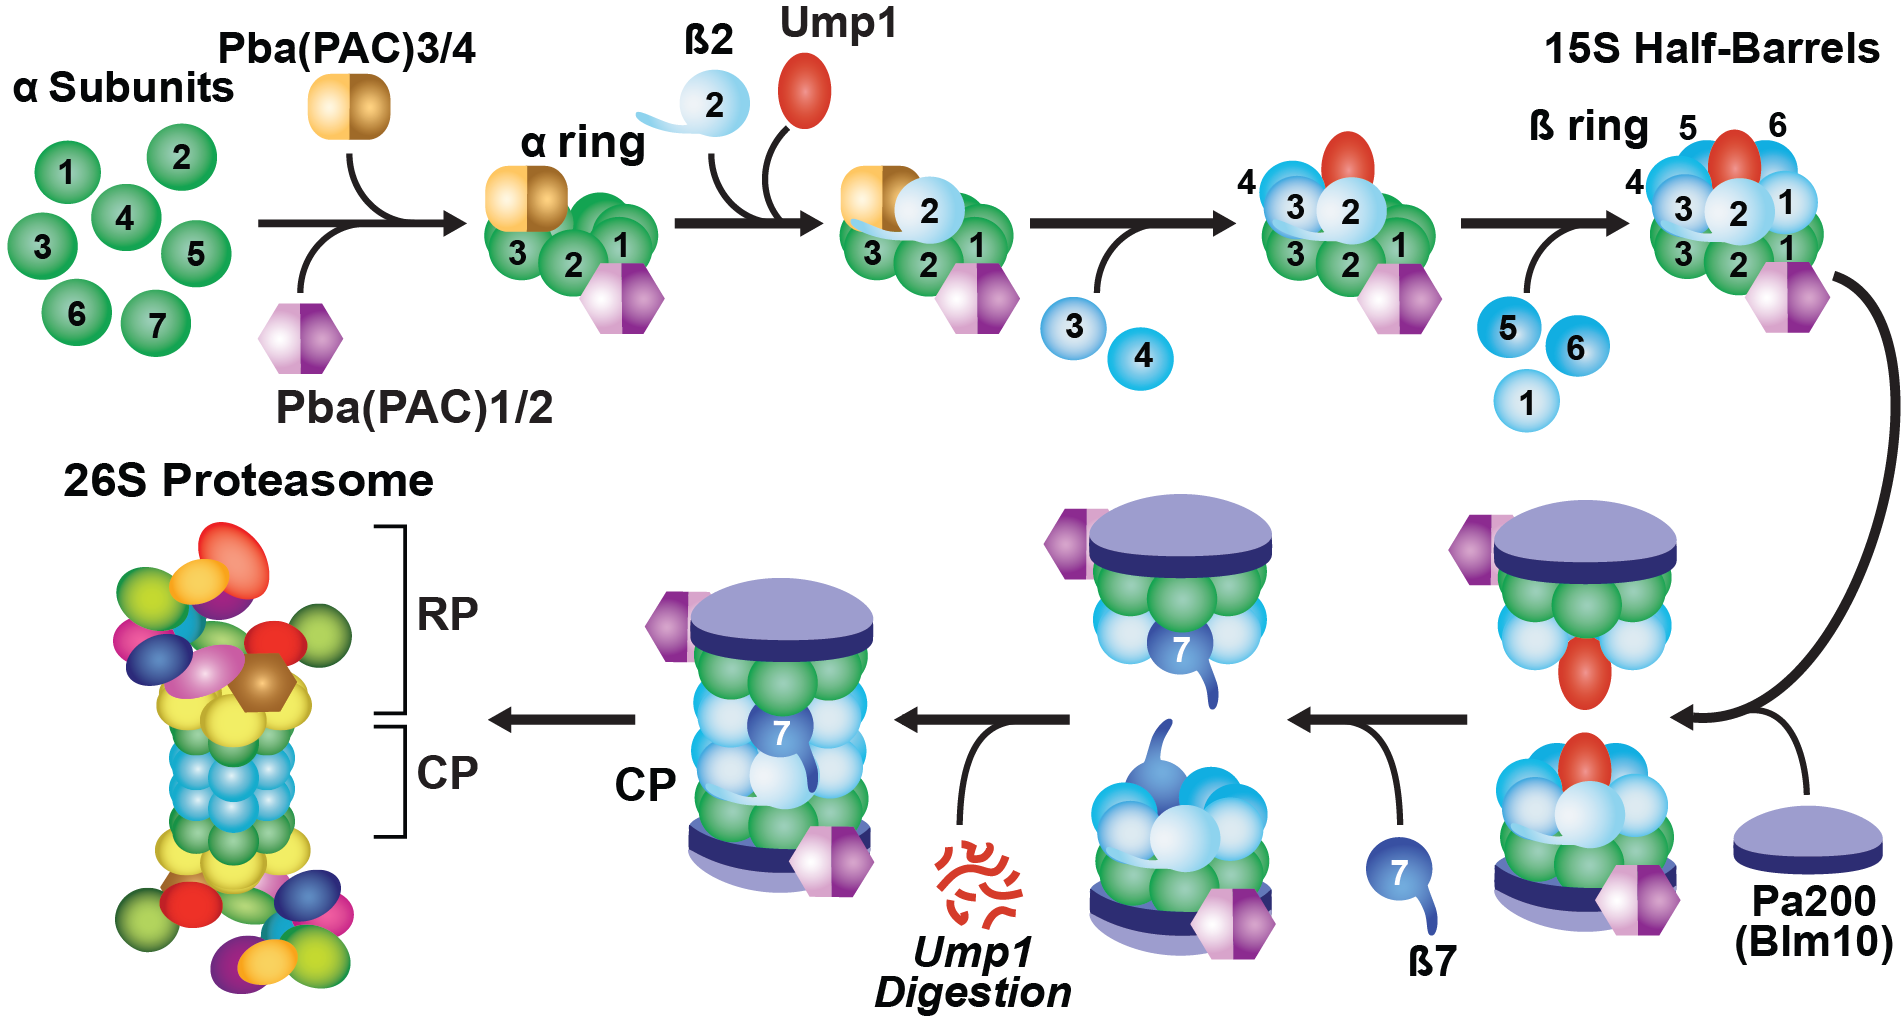
\includegraphics[width=\columnwidth]{intro/cpassembly.png}
	\mycaption{Schematic representation of CP Assembly}
	{Adapted from \citep{hirano08}. Pba1-4 (yeast) and PAC1-4 (human) nomenclature is used. Free $\alpha$-subunits are bound to prevent aberrant $\alpha$-ring assembly by Pba1-4. The $\beta$2 subunit along with Ump1 bind this $\alpha$-ring, and subsequently the Pba(PAC)3/4 heterodimer leaves the assembly complex. Then the $\beta$3 and $\beta$4 subunits are incorporated and the $\beta$5 and $\beta$6 subunits are added forming a 15S half-barrel, possibly with the help of PA200. Two half-barrels come together and the last $\beta$-subunit, $\beta$7 is added. N-terminal propeptides for $\beta$-subunits are autocatalytically cleaved, Ump1 is degraded as the first substrate of the nascent proteasome, and a fully functional CP is generated.}
	\label{fig:cpassembly}
\end{sidewaysfigure}
 
	An additional suite of assembly chaperones aide in construction of the CP including the proteasome biogenesis associated Pba1-4 proteins in yeast, and the proteasome assembly chaperones PAC1-4 in mammals. The yeast assembly chaperones Pba1 and Pba2 were initially discovered in affinity preparations of the CP in a genetic background that induced the formation of aberrant 15S half-barrels \citep{li07}. MS/MS analyses of these 15S complexes separated by native-PAGE identified Pba1, Pba2, and Ump1 contained in these complexes suggesting that Pba1 and Pba2 played a role in CP assembly \citep{li07}. In a separate study, Pba1 and Pba2, along with two additional assembly chaperones Pba3 and Pba4 were identified in a mutant screen for suppressors of a conditional dominant lethal allele of Rad53 which induces DNA damage \citep{le07}. Pba1, and Pba2 were found to co-fractionate with both the precursor propeptide form of the $\beta$2 subunit, and the mature form; however, Pba3 and Pba4 were found to exclusively fractionate with the propeptide form of $\beta$2 \citep{le07}. These data suggested that Pba3 and Pba4 aided in earlier stages of assembly, while Pba1 and Pba2 seemed to act at both early and later stages. Pba1 and Pba2 were found to form a heterodimer, while Pba3 and Pba4 were found to form a separate heterodimer \citep{le07}.
	
	An orthologous system to the yeast Pba1-4 system was elucidated in mammals. PAC1 and PAC2 were first identified in affinity preparations of an immature propeptide form of the $\beta$1 subunit, and like their yeast counterparts (Pba1 and 2) were found to form a stable heterodimer \citep{hirano05}. Consistent with their role in assembly they were found to co-fractionate with immature $\beta$-subunits, and Ump1 \citep{hirano05}. Overexpression of these PAC1 and PAC2 chaperones yielded increases in half- barrel precursors, while knockdown by siRNA impaired assembly of the CP complex \citep{hirano05}. An additional chaperone involved in assembling the $\alpha$-ring was identified in PAC1 immunopurifications in human cell lines, and was termed PAC3 \citep{hirano06}. siRNA knockdown of PAC3 attenuated $\alpha$-ring formation and gave rise to the accumulation of free $\alpha$-subunits, suggesting that PAC3 played a role in stabilization of the CP $\alpha$-ring \citep{hirano06}. Mammalian PAC4 was identified as an ortholog to yeast Pba4 through PSI-BLAST analyses \citep{kusmierczyk08} and together with PAC4 forms a heterodimer, like its yeast Pba3/4 counterpart \citep{le07}.
	
	The role of the PAC1/2 and PAC3/4 heterodimers in assembly, along with the exact ordered incorporation of $\beta$-subunits was aided by siRNA knockdown of specific $\beta$-subunits, and studying the resulting assembly products \citep{hirano08}. Through this analysis Hirano \textit{et al}. clearly delineated PAC3/4's role in early assembly, and found that PAC3 and PAC4 must leave the assembling half-barrel before the addition of the $\beta$3 subunit. While this was demonstrated in mammals, observations of the yeast Pba3/4 heterodimer suggest a similar model in which the Pba3/4 heterodimer also remains bound to the $\alpha$-ring until the $\beta$2 subunit binds \citep{kusmierczyk08, yashiroda08}. While Pba(PAC)3/4 act early in assembly, Pba(PAC)1/2 have the propensity to bind the mature proteasome, and stay bound even after the incorporation of $\beta$-subunits.
	
	A model of yeast and mammalian assembly adapted from Hirano \textit{et al}. is as follows (Figure \ref{fig:cpassembly}).  After the $\alpha$-ring is formed, with the help of Pba(PAC)1/2 and Pba(PAC)3/4, the $\beta$2 subunit is incorporated along with its C-terminal tail that helps to recruit the $\beta$3 subunit \citep{hirano08}. Pba(PAC)3/4 is released upon $\beta$3 subunit binding \citep{hirano08}. Ump1 stabilizes the incorporation of additional $\beta$-subunits by binding their inherently disordered propeptide regions \citep{li07}. $\beta$4, $\beta$5, $\beta$6, and $\beta$1 are then incorporated \citep{hirano08}. At this stage PA200 may help stabilize this precursor; however, its exact role in assembly is poorly understood.  Two 15S half proteasomes come together, and finally the $\beta$7 subunit is incorporated \citep{hirano08}. The $\beta$-subunit propeptides are then cleaved exposing the catalytically active N-terminal threonines and Ump1 is degraded becoming the first substrate of the nascent CP \citep{li07}. Pba(PAC)1/2 are then released, or can bind mature proteasomes until activation by the RP \citep{hirano08}. Taken together these data are consistent with a model in which the heterodimeric pair Pba(PAC)3/4 acts at early stages to assemble free $\alpha$-subunits into an $\alpha$-ring while preventing the formation of aberrant $\alpha$-subunit complexes \citep{hirano08}. In contrast, the heterodimeric pair Pba(PAC)1/2 acts at both early and later stages in proteasome assembly and has the ability to bind mature CP \citep{wani16}.
	
	While the CP assembly process is conserved in yeast and mammals, the orthologs involved share very little sequence homology. The Ump1 orthologs share \textasciitilde{}20\% identity, and Pba1-4 and PAC1-4 share \textasciitilde{}10\% identity respectively \citep{murata09}. Despite this low sequence identity, structural analysis revealed that the Pba3/4 heterodimer shared significant structural features with the human PAC3 protein, suggesting that these assembly chaperones may have retained structural similarities \citep{yashiroda08}. The Hochstrosser group also speculated that the Pba1/2 and PAC1/2 complexes may be structurally related \citep{kusmierczyk11}. Besides these speculative structural implications, Pba1 and Pba2 share some protein sequence features, including HbYX motifs important for their interaction with the $\alpha$-ring \citep{kusmierczyk11}. These features are conserved in their mammalian orthologs with PAC1 containing a HbYX motif, while PAC2 shares a HbYX-like HbY/F motif that is conserved in other eukaryotes outside the fungal kingdom \citep{kusmierczyk11}.
	
	Structural analysis of these CP assembly chaperones have also provided insight into their function. Pba1, and Pba2 were able to bind mature 20S proteasomes, and a co-crystal structure has been solved by X-ray crystallography \citep{stadtmueller12}. The HbYX motif found in Pba1 was shown to intercalate between the $\alpha$5 and $\alpha$6 subunits, while the HbYX motif found in Pba2 was shown to intercalate between the $\alpha$6 and $\alpha$7 subunits (Figure \ref{fig:pba12hbyx}). Crystal structures of the Pba3, Pba4 complex were shown to be similar to the PAC3 suggesting similar role \citep{yashiroda08}. A co-crystal structure binding the $\alpha$5 subunit helped define the binding surface of the Pba3/4 heterodimer \citep{yashiroda08}. This binding surface for Pba3/4 occurs on the opposite side of the $\alpha$-ring as compared to the Pba1/2 binding surface providing further structural evidence for the distinct and separate roles that the Pba1/2 and Pba3/4 play in proteasome assembly (see Figure \ref{fig:pba14structure}) \citep{stadtmueller12, yashiroda08}.

\begin{figure}[p]
	\scalebox{.5}{
	\centering
	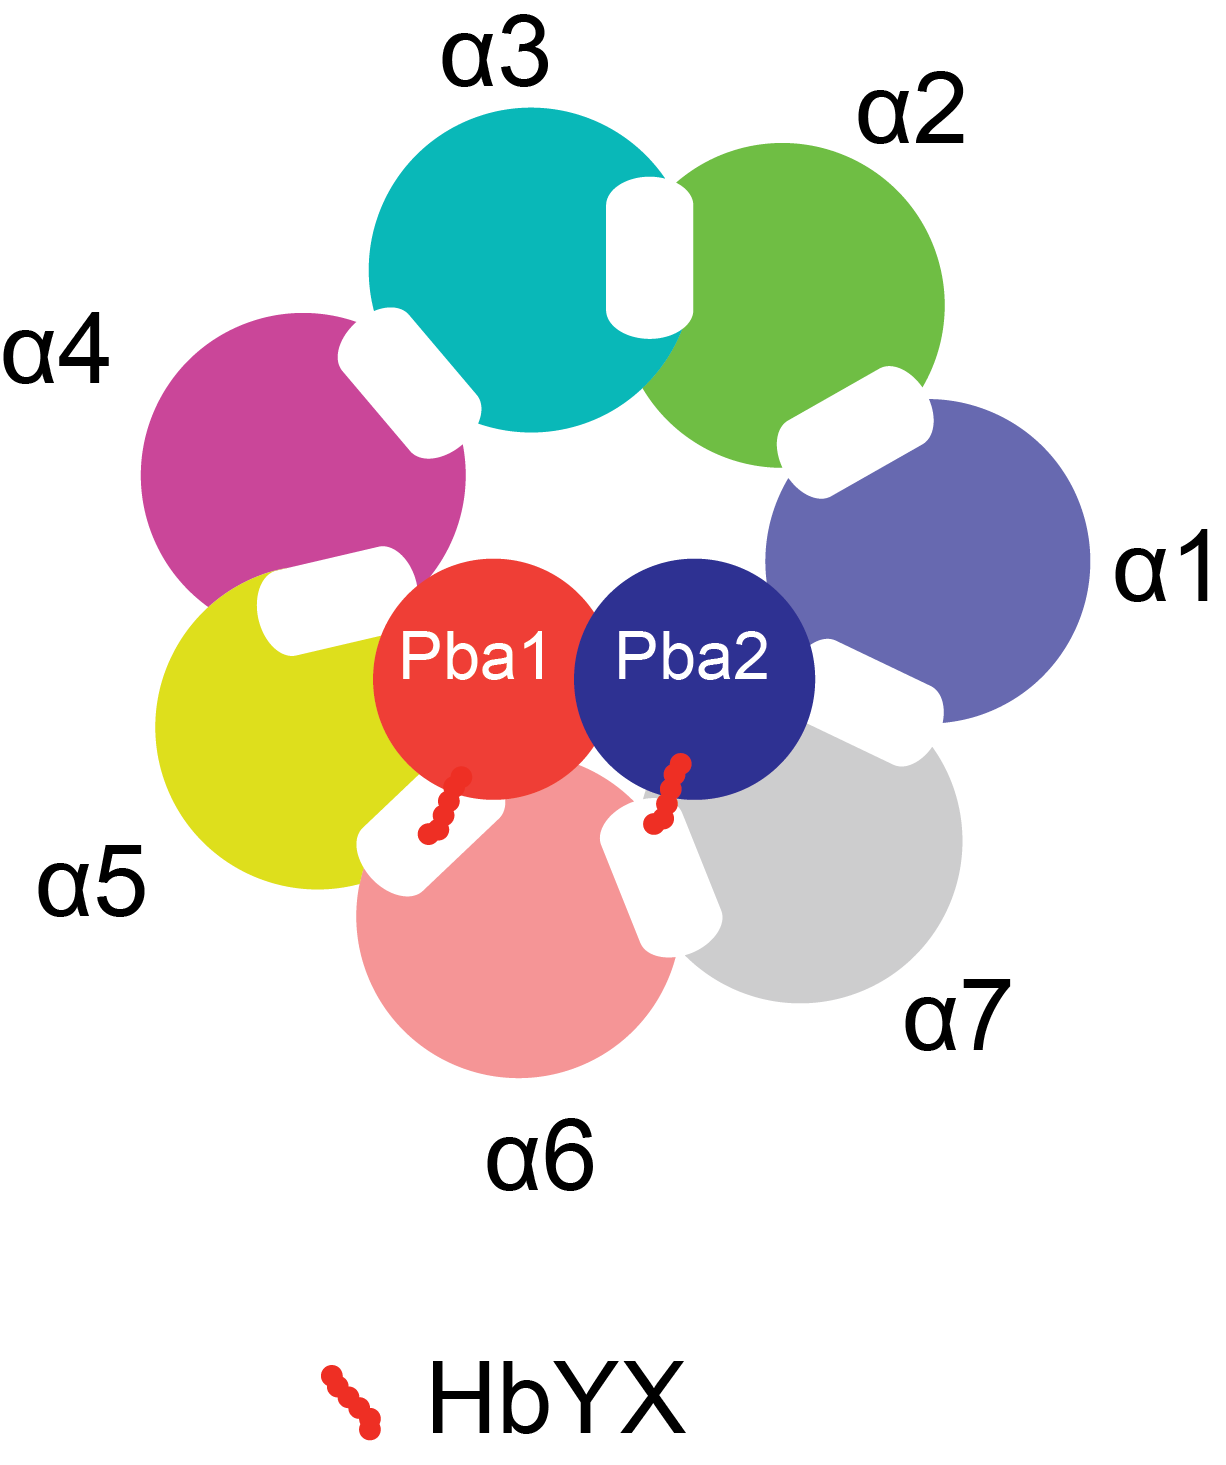
\includegraphics[width=\columnwidth]{intro/pba12hbyxbinding.png}}
	\mycaption{Pba1 and Pba2 binding sites via their HbYX motifs into adjacent $\alpha$-subunit pairs}
	{$\alpha$-ring is shown with adjacent Pba1 and Pba2 binding surfaces that intercalate between $\alpha$-subunits. Pba1 intercalates between $\alpha$5 and $\alpha$6, while Pba2 intercalates between $\alpha$6 and $\alpha$7 \citep{yashiroda08}.}
	\label{fig:pba12hbyx}
\end{figure}

\begin{FPfigure}[Figure \ref{fig:pba14structure} \textit{caption follows on next page}]
	\centering
	\includegraphics[width=\columnwidth]{intro/pba14structure.png}
	\mycaption{Structural Diagram of opposing Pba1/2 Pba3/4 binding}
	{Structures were obtained from the Protein Data Bank with PDB ID 4G4S for Pba1 and Pba2 bound to yeast 20S proteasome \citep{stadtmueller12}, and PDB ID 2Z5C for Pba3 and Pba4 bound to the $\alpha$5 subunit\citep{yashiroda08} and visualized using PyMOL \citep{PyMOL}. The $\alpha$5 subunit was used to align the structures so that the opposing Pba1/2 and Pba3/4 interfaces could be visualized in reference to the 20S $\alpha$-ring. \textbf{(A)} 20S $\alpha$-ring with alone (left), Pba1/2 heterodimer, and Pba3/4 heterodimer alone (middle), and 20S $\alpha$-ring with bound Pba1-4 shows the opposing binding surfaces, with Pba1/2 binding to the top of the $\alpha$-ring, and Pba3/4 binding to the bottom of the $\alpha$-ring where $\beta$-subunits normally bind in the full 20S proteasome. \textbf{(B)} $\alpha$-ring with Pba1/2 binding. \textbf{(C)} $\alpha$-ring with Pba3/4 binding. \textbf{(D)} Binding of Pba3/4 prevents premature binding of the $\beta$-ring (shown as a grey ribbon structure), specifically to occlude the $\beta$3 subunit \citep{yashiroda08}.}
	\label{fig:pba14structure}
\end{FPfigure}
	
	Outside of eukaryotes, proteasome assembly has also been studied in \textit{archeal} and \textit{eubacterial} proteasome models \citep{kusmierczyk11}. While the assembly of these proteasomes can occur without assembly chaperones two chaperones, PbaA and PbaB were identified that likely aide in efficient assembly of the particle \citep{kusmierczyk11}. PbaA and PbaB are evolutionarily related to yeast Pba1 and Pba2 and both harbor conserved HbYX motifs showing that these chaperones provide an ancient link to proteasome assembly evolution \citep{kusmierczyk11}.
\FloatBarrier
\subsection{19S Regulatory Particle Assembly – RP base}
	Like the chaperones that facilitate CP assembly, there are proteins that aide in proper formation of the RP. The majority of identified RP assembly chaperones are involved in the assembly of the RPT base ring. The RP base assembly chaperone Hsm3 was identified in the same screen for suppressors of Rad53 that identified the yeast CP assembly chaperones Pba1-4 \citep{le07}, although HSM3 was not characterized until two years later \citep{le09}. Several months later additional RP assembly chaperones (Nas2, Nas6 and Rpn14) were identified and characterized as components of an RP base assembly system \citep{funakoshi09}. The majority of these RP base chaperones function by binding the C-terminal domains of RPT subunits preventing them from forming pre-mature contacts with the CP \citep{funakoshi09}. However, their evolutionary history is likely distinct as they are made up of distinct domains including ARM/HEAT repeats in Hsm3, coiled-coil PDZ domains in Nas2, ankyrin repeats in Nas6, and WD40 repeats in Rpn14 \citep{funakoshi09}.

	Immunoprecipitation of Hsm3 showed that it interacted with several RP base subunits; however no $\alpha$-subunits or RP lid subunits were detected suggesting that Hsm3 may be specific to the RP base \citep{le09}. Fractionation of crude protein lysates from yeast showed that Hsm3 associated with free RP but not with the mature 26S proteasome, suggesting  that it may be involved in RP assembly \citep{le09}. Assembly intermediates containing Hsm3, Rpn1, and Rpt2 were identified when RP base assembly was impaired \citep{funakoshi09}.  A mammalian ortholog of Hsm3, HSM3 was found to form a similar complex in mammals \citep{kaneko09}. Recently, a co-crystal structure involving Hsm3, Rpt1, and Rpt2 showed that Hsm3 forms contacts with the C-terminal domains of both Rpt1 and Rpt2, providing further support for the formation of this pre-assembly complex and that these assembly chaperones function to prevent premature binding of the C-terminus of RPT subunits to the CP \citep{barrault12}.

	As described above, the C-terminal domains of RPT subunits contain HbYX motifs, which are important for binding the $\alpha$-ring. Mutating the HbYX motif of either Rpt4 or Rpt6 by removing a single amino acid was sufficient to induce the formation of two separate pre-assembly complexes with one containing Hsm3 Rpn1, and Rpt1, 2, and 5 and another containing Rpn14, Rpt4, and Rpt6 \citep{park09}. The formation of these pre-assembly complexes was blocked in triple null mutants for Hsm3, Bas6 and Rpn14 \citep{park09}. Interestingly single mutants in either Nas6, or Rpn14 did not exhibit strong assembly defects; however, yeast deficient in both Nas6, and Rpn14 exhibited a strong assembly defect suggesting that Nas6, and Rpn14 play semi-redundant roles \citep{saeki09}. Despite this redundancy MS/MS analyses of tagged assembly chaperones and yeast-two-hybrid analyses showed Nas6 binding predominantly to Rpt3, while Rpn14 was found to predominantly bind to Rpt6 \citep{saeki09}.  The yeast Nas2 assembly chaperone was found to bind to Rpt5, and its mammalian ortholog NAS2 was shown to form a complex with both RPT4 and RPT5. Recent structural analyses of Nas2 suggest that it binds the C-terminus of Rpt5 likely acting to prevent pre-mature binding with the CP \citep{satoh14}.

	A general model emerges in which a majority of the RP base assembly chaperones act to prevent pre-mature association of unassembled RP base by actively binding the C-termini of RPT subunits \citep{tomko13}. This model involves four separate modules including [Hsm3 with Rpn1, Rpt1, and Rpt2], [Nas2 with Rpt4, and Rpt5], [Nas6 with Rpt3], and [Rpn14 with Rpt6].  While the exact ordered steps of RP base assembly are still unclear, the process appears to be conserved between both yeast and mammals. A model of RP base assembly using the yeast nomenclature is presented in Figure \ref{fig:rpassembly} showing how the individual modules may come together to form the RP base.

\begin{sidewaysfigure}[p]
	\centering
	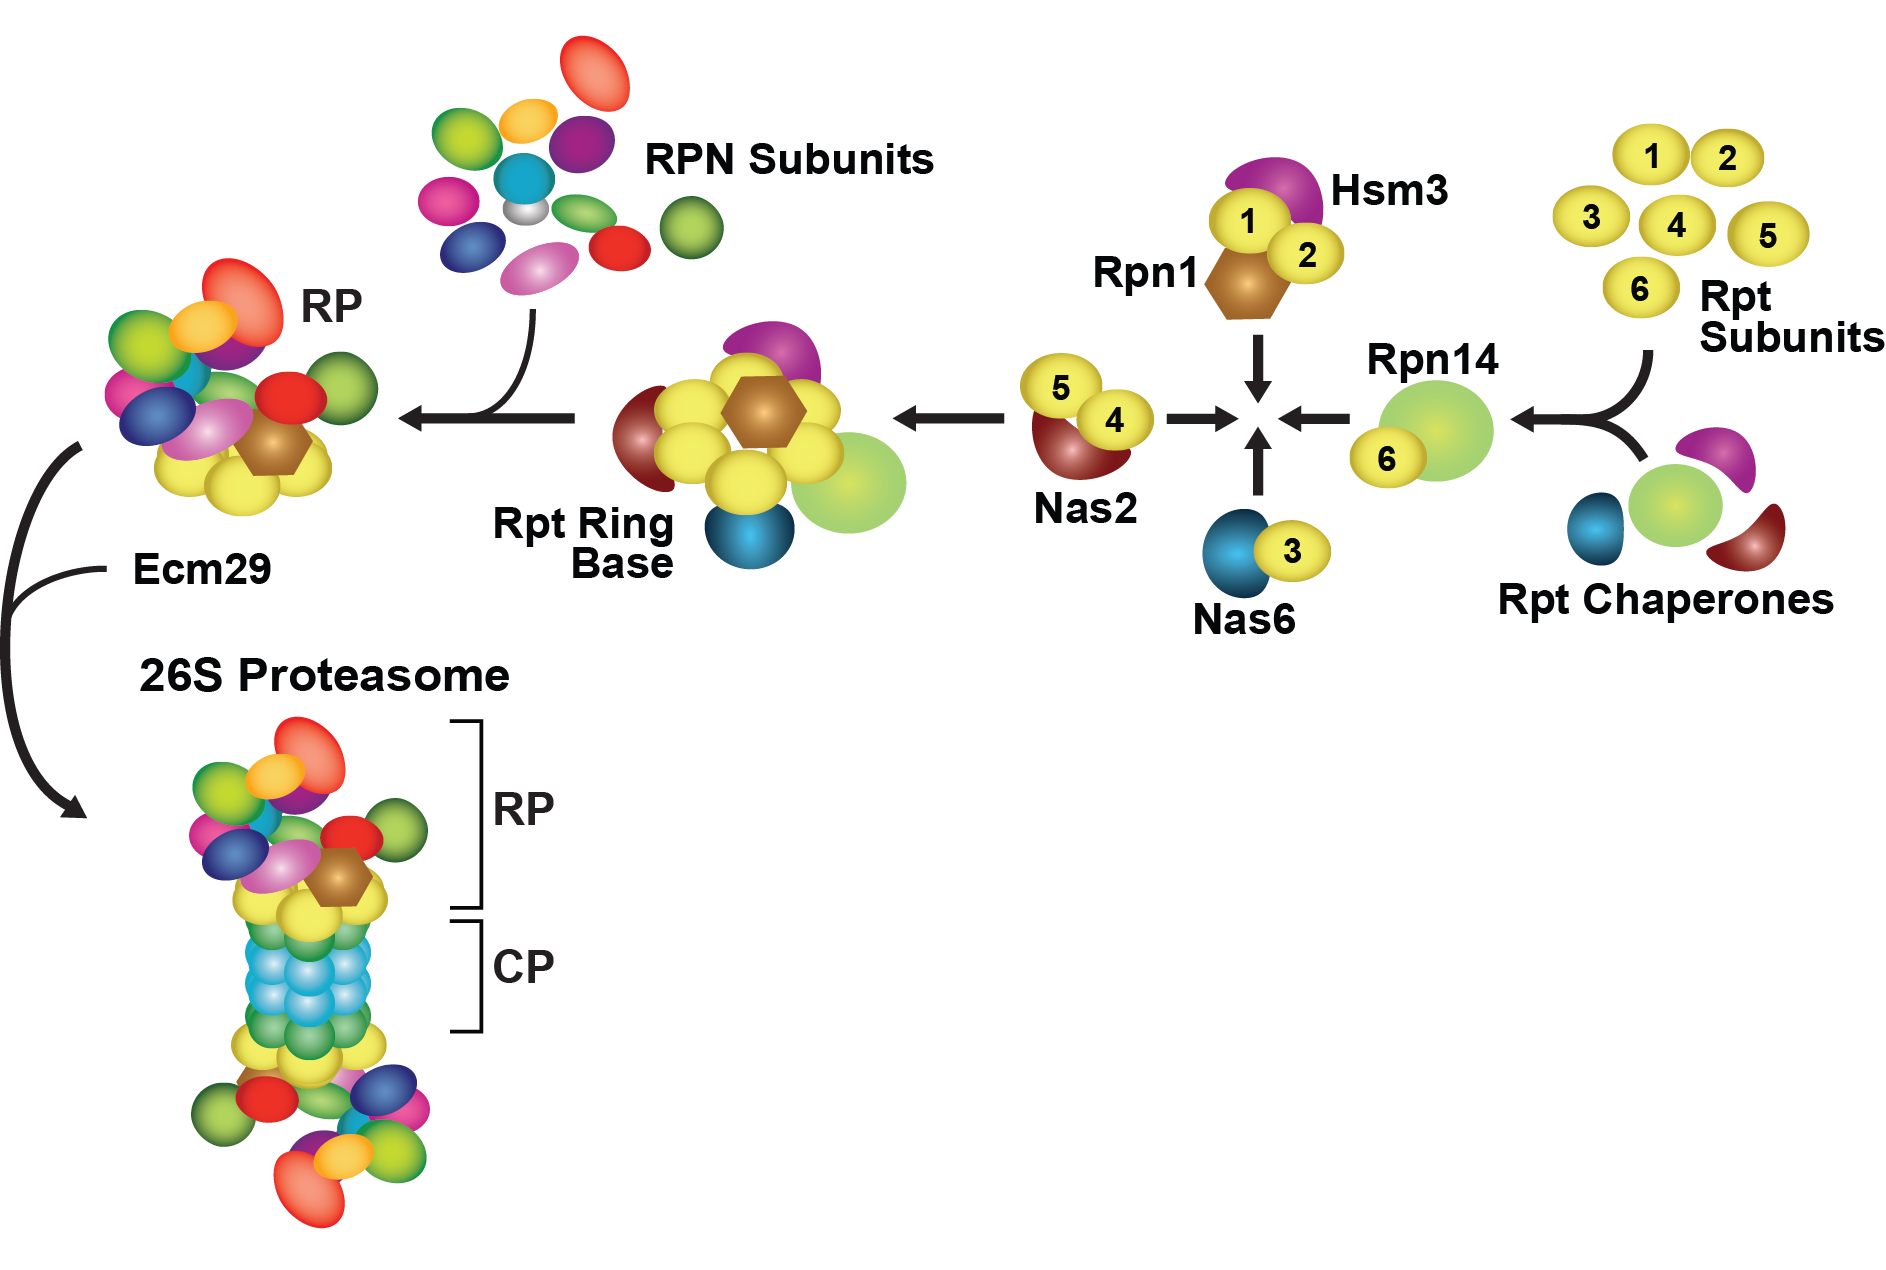
\includegraphics[width=\columnwidth]{intro/rpassembly.png}
	\mycaption{Schematic representation of RP Assembly}
	{While the exact order of RP-base assembly is unclear, it involves several modules including [Hsm3 with Rpn1, Rpt1, and Rpt2], [Nas2 with Rpt4, and Rpt5], [Nas6 with Rpt3], and [Rpn14 with Rpt6].}
	\label{fig:rpassembly}
\end{sidewaysfigure}

\subsection{19S Regulatory Particle Assembly – RP lid}
	Several modules and chaperones are involved in the assembly of the RP base; however, construction of the RP lid is not well understood. RP lid assembly has primarily been investigated in yeast by mutant analyses of specific RP lid subunits including mutants in Rpn7, Rpn9 and Rpn12 \citep{fukunaga10}. MS/MS analyses of affinity purified lid complexes in these differing mutant backgrounds identified two different subassemblies, the first containing Rpn5, 6, 8, 9, and 11, and the second containing Rpn3, Rpn7, and Sem1 \citep{fukunaga10}. Intriguingly, Sem1 was found to act as a bridge between Rpn3, and Rpn7, as cleavage of an engineered version of Sem1 containing a Tobacco Etch Virus (TEV)-cleavage site showed defects in RP lid assembly \citep{tomko14}. While Sem1 may play a role in proteasome biogenesis, alternative roles for Sem1 have been proposed.  In the mature particle, Sem1 has been found to aide in recognition of ubiquitin chains which are linked at lysine 48 or 63 \citep{paraskevopoulos14}. Proteasomes affinity purified from Sem1 mutants had only mild defects in stability, suggesting that its main function may be that of ubiquitin recognition \citep{paraskevopoulos14}.
	
	Structural studies of the RP lid, have identified conserved C-terminal helices that form a helical bundle important in assembly of this sub-complex \citep{estrin13}. The assembly of the lid was investigated by expressing the full complement of yeast RP lid subunits in which the C-terminal helices were removed in varying combinations \citep{estrin13}. In the most extreme case, when the RPN6 helical bundle was omitted, a similar arrangement as described above was identified with four distinct sub-complexes identified that included [Rpn5, 8, 9, and 11], [Rpn3, and Rpn7], [Rpn6 alone], and [Rpn12 alone] \citep{estrin13}. Estrin \textit{et al}. speculate on the exact ordering of the assembly, but this has not been thoroughly investigated.

	While the exact ordering involving the other RP lid subunits is unclear, RPN12 is likely the last subunit to be added to the RP lid. In Rpn9 mutant cells, Rpn12 was completely absent from the RP lid \citep{fukunaga10}. However, mutants in Rpn12 exhibited the full complement of RP lid subunits suggesting that Rpn12 was likely the last subunit added to the RP lid \citep{tomko11}. The conserved C-terminus of RPN12 was found to contact both the RP base and lid suggesting that RPN12 might be a final checkpoint for RP lid and base assembly \citep{tomko11}. When the RP lid helical bundle described above is impaired, RPN12 cannot bind, suggesting a mechanism by which RPN12 can scan this bundle for proper assembly \citep{estrin13}.
	 
\subsection{RP-CP Assembly and Alternative Capping Particles}
 	While there are dedicated chaperones for the CP and RP, an additional chaperone mediates assembly of the final particle \citep{ramos98}.  ECM29 stabilizes the association of assembled CP and RP and provides a final quality control checkpoint for mature 26S proteasomes \citep{besche14, lehmann10}.  
	Finally, in some situations, the RP is replaced entirely by alternate capping particles such as PA200 (also known as Blm10) or CDC48 \citep{barthelme12, book10, schmidt05}.  The functions of these caps are not yet clear, but recent proposals for PA200 have it participating in 26S proteasome assembly, helping shuttle proteasomes into the nucleus, and/or generating a ubiquitin-independent proteasome containing CP and PA200 only \citep{dange11, sadre-bazzaz10, weberruss13}. However, in plants, mutants in PA200 exhibit no gross morphological defects showing that PA200 is not essential to plant growth and development \citep{book10}.

\subsection{Proteasome Assembly in Plants}
	While much is known about proteasome assemble in both yeast and mammals, very little is known about how plants assemble this particle. There is some evidence that plants likely use a similar process as an ortholog of PAC2, PBAC2, has been identified in affinity preparations for the plant CP complex \citep{book10}. A slightly different normenclature is used in plants as compared to Pba in yeast and PAC in mamamls as both of these can refer to proteasome $\alpha$- and $\beta$-subunits (example, $\alpha$1 is PAC1, and $\beta$1 is PBA1 in \textit{Arabidopsis}). Furthermore, PSI-BLAST-based bioinformatic analyses, similar to the one used to find orthologs between yeast and humans was able to identify some putative plant orthologs (PBAC1 and PBAC2) to the mammalian PAC1 and PAC2 assembly chaperones by two separate research groups, although their annotations in The \textit{Arabidopsis} Information Resource (TAIR) are incomplete \citep{kusmierczyk11, le07}. These identified orthologs share very little sequence identity (<10\%), although this is unsurprising given the poor sequence identity between the yeast and mammalian orthologs \citep{kusmierczyk11, le07, murata09}.  Genomic searches based on BLAST alone, have failed to identify orthologs of the CP assembly chaperones; however putative orthologues for NAS2, NAS6, and HSM3 are readily identifiable in the genome (Chapter 3).  Together these data suggested that our analysis of plant proteasome assembly has remained incomplete. One goal of this thesis, explored in Chapter 3, was to identity additional CP and RP interacting proteins, potentially including some of these assembly chaperones.

\section{Proteasome Isotypes}
	In yeast, proteasome subunits are typically encoded as a single subunit, however in animals specific subunits are replaced to form different proteasome isotypes. This replacement typically occurs due to tissue specific expression of alternative CP subunits. Several examples of isotypes exist, including the Immunoproteasome, the thymoproteasome proteasome, and the testes-specific proteasome.

\subsection{Immunoproteasome}
While the proteasome was first discovered in the 1970's it wasn't until 20 years later that an alternative form of the proteasome, the immunoproteasome was discovered \citep{brown91, glynne91, ortiz-navarrete91}. The immunoproteasome was discovered while trying to determine how small antigen presenting peptides are produced for the major histocompatibility complex (MHC). The MHC is a set of cell surface proteins involved in the acquired immune response (reviewed in \citep{neefjes11}). Small peptides resulting from normally present cytosolic proteins (MHC class I antigens) are loaded into the MHC and presented on a cell's surface helping establish a normal profile of surface peptides recognized by the immune system. Atypical protein production, whether through viral or bacterial infection, or by cells that are proliferating abnormally, such as cancerous cells, result in atypical surface peptides causing the immune system to respond and recruit CD8+ T-killer cells to remove the aberrant cell. Several of the identified genes involved in this process were termed low molecular weight proteins, or LMPs and their protein sequences were found to be related to the proteasome. The cytokine Interferon-gamma, a small signaling protein involved in the immune response was found to induce expression of three alternative $\beta$-subunits of the proteasome ($\beta$1i, $\beta$2i, and $\beta$5i), which are then incorporated to form the immunoproteasome (Figure \ref{fig:proteasomeisotypes}) \citep{aki94, groettrup96}.

\begin{figure}[p]
	\centering
	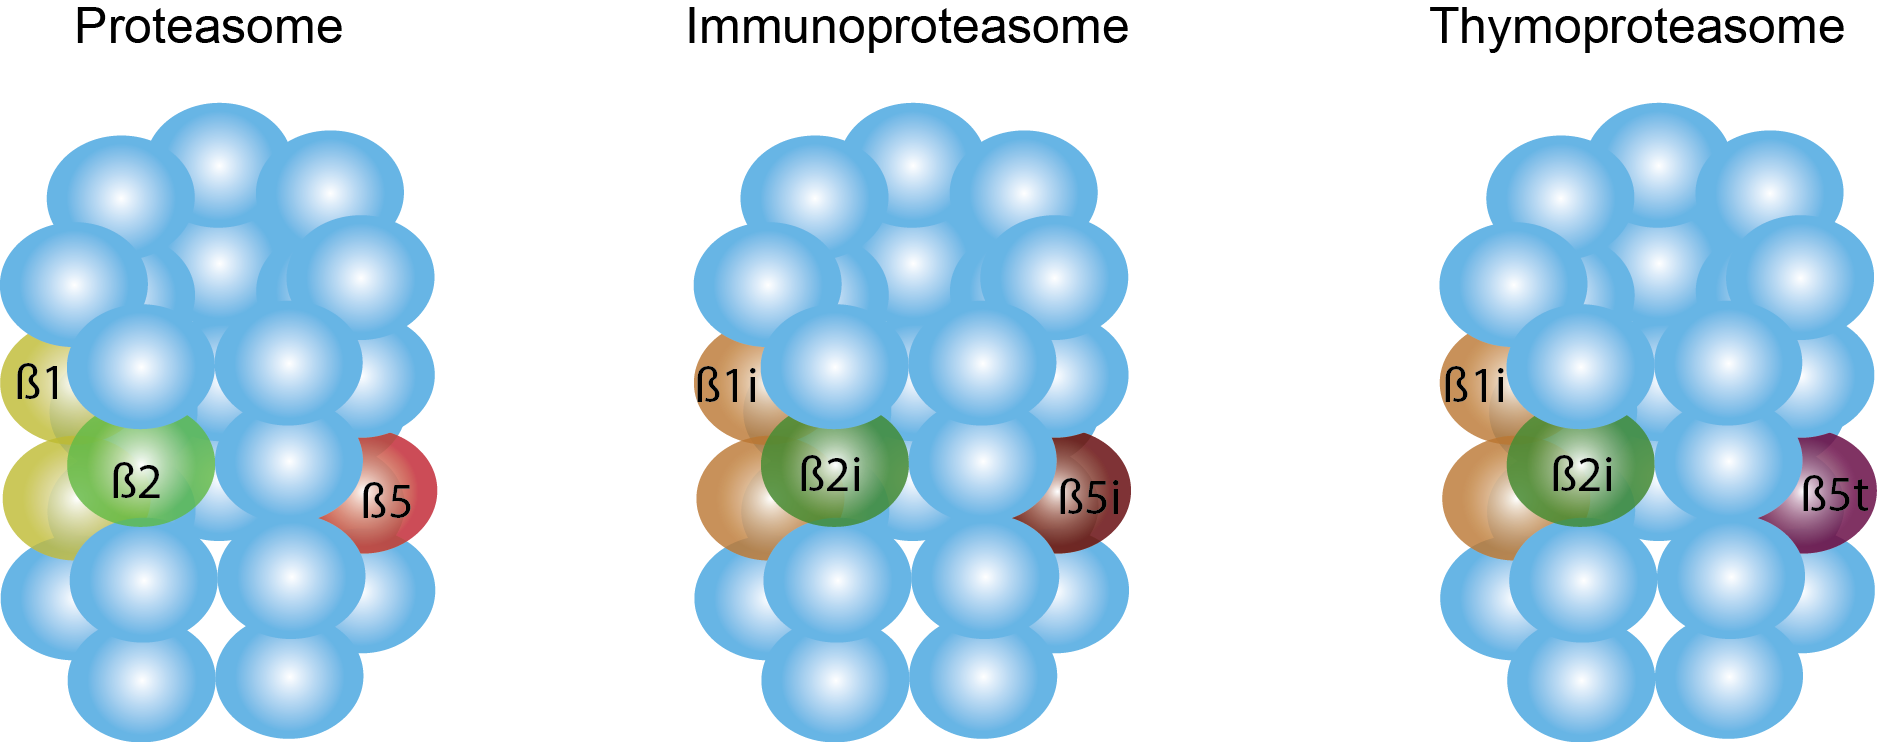
\includegraphics[width=\columnwidth]{intro/proteasome_isotypes.png}
	\mycaption{Representation of subunits replaced for both the immunoproteasome and the thyoproteasome}
	{Adapted from \citep{groettrup09}. The three catalytically active sites of the proteasome $\beta$1, $\beta$2, and $\beta$5 are replaced with the immunoproteasome variants $\beta$1i, $\beta$2i, and $\beta$5i. Furthermore, in the thyoproteasome the $\beta$5i subunit is replaced with another variant the $\beta$5t subunit.}
	\label{fig:proteasomeisotypes}
\end{figure}

An elegant study that compared the enzymatic activity of affinity purified 20S proteasomes with immunoproteasomes using model peptide substrates determined that cleavage after acidic residues via the $\beta$1's PGPH activity is nearly eradicated by the replacement of the $\beta$1 subunit with the immunoproteasome $\beta$1i's subunit which favors chymotryptic activities \citep{dahlmann00}. Together these altered enzymatic activities allow for the production of peptides more favorable for antigen presentation to the MHC. 

\subsection{Thymoproteasome proteasome}
	A sub-type of the immunoproteasome was discovered in the thymus. A search for proteasome related genes identified an uncharacterized ortholog of the $\beta$-subunit that was preferentially expressed in thymus tissue, termed $\beta$5t \citep{murata07}. This thymoproteasome was similar in composition to the immunoproteasome in that it contained the altered $\beta$1i, and $\beta$2i subunits; however, the $\beta$5i subunit was replaced with this novel $\beta$5t subunit (shown in Figure \ref{fig:proteasomeisotypes})  \citep{murata07}. Expression of the $\beta$5t was even further sub-localized to cells in the thymic cortex, and mice lacking this subunit could not generate CD8+ T cells, normally involved in aiding in the destruction of foreign invaders \citep{murata07}. 

\subsection{Testes-specific proteasome}
	Like the discovery of the thymoproteasome proteasome, the discovery of the testes-specific isotype was initially driven by a bioinformatics search for proteasome related genes \citep{uechi14}. A search revealed an uncharacterized ortholog of the $\alpha$4 subunit that shared 85\% amino acid identity, termed here $\alpha$4s \citep{uechi14}. Analysis of $\alpha$4s's expression by qRT-PCR analysis showed that it was expressed in all tissues; however only $\alpha$4s protein accumulated in testes \citep{uechi14}. $\alpha$4s is preferentially incorporated over the $\alpha$4 subunit in testes, however $\alpha$4s specific proteasomes did not show altered enzymatic activities, and its biological function remains unknown \citep{uechi14}.  

\subsection{$\alpha$4-$\alpha$4 proteasome Isotype}
	When defects are present in the Pba(PAC)3/4 heterodimer the $\alpha$3 subunit is replaced by the $\alpha$4 subunit, making an $\alpha$4-$\alpha$4 specific proteasome isotype \citep{kusmierczyk08, padmanabhan16}.  Intriguingly, this $\alpha$4-$\alpha$4 isotype occurs in both mammals and yeast, conferring increased resistance to heavy metal ions, suggesting an evolutionarily conserved role for these proteasome isotypes \citep{kusmierczyk08, padmanabhan16}.  Additionally, $\alpha$4 levels are modulated by several oncogenes including BRCA1 \citep{li15}, and the formation of these alternative subtypes is highly dependent on the relative availability of $\alpha$3 vs $\alpha$4. Together these data suggest that $\alpha$4-$\alpha$4 proteasome isotypes may play a role in the progression of cancer \citep{padmanabhan16}.
\FloatBarrier
\subsection{Plant Proteasome Isotypes}
	Outside of the proteasome isotypes discussed above, animal and yeast genomes typically encode a single gene for most proteasome subunits. In rice the RPT family has been duplicated such that four of the six RPT subunits are encoded as paralogs \citep{shibahara04}. While the function of these duplicated subunits is unclear, they do exhibit alternative tissue specific expression patterns as determined by MS/MS analyses using total protein extracts. Specifically, the expression patterns differed between bran and callus suggesting that there is tissue specific regulation of these sets of RPT subunits. 
In the most extreme case, most subunits in \textit{Arabidopsis} are encoded as paralogs, likely due to a genome duplication \citep{book10, fu98}. MS/MS analyses of proteasomes purified from \textit{Arabidopsis} showed that most of these subunit paralogs are incorporated into the proteasome. Therefore, \textit{Arabidopsis} has the propensity to assemble its proteasomes into a diverse array of proteasome isotypes by incorporating specific subsets of isoforms. Some genetic evidence exists that suggests that these paralogs may have differing functions. RPN1a and RPN1b play differing roles in embryogenesis \citep{brukhin05}, and overexpression of RPN5a induces an early senescent phenotype while overexpression of RPN5b does not \citep{book09}.  Despite these observations, it is unclear if plants assemble their proteasome subunit isoforms into compositionally and functionally distinct isotypes. One of the objectives of this thesis was to determine if \textit{Arabidopsis} can assemble proteasome isotypes by leveraging label-free quantitative mass spectrometric analysis of affinity preparations enriched for either the RPT4a or RPT4b subunit isoforms (explored in Chapter 3). If plants can assemble distinct isotypes, preparations for either isoform may show enrichment for other subunit isoforms; however, if plants assemble its subunit isoforms in a random fashion the preparations should be similar. 


\section{Conclusions}
The \textit{Arabidopsis} 26S proteasome exists \textit{in planta} as a diverse array of complexes containing multiple subunit isoforms and interacting proteins \citep{book10, fu99, yang04}. However, there are several gaps in our knowledge of the plant particle.  While the yeast and mammalian CP assembly systems are well described, very little is known about proteasome assembly in plants. Initial MS/MS analyses of the plant complex identified a likely ortholog related to PAC2, named PBAC2, suggesting that the plant system may be similar; however, no additional assembly chaperones were described \citep{book10}. Several putative \textit{Arabidopsis} assembly orthologs were identified through PSI-BLAST analyses including orthologs for PAC1, and PAC2 by both the Hoschstrasser group, and others \citep{kusmierczyk11, le07}; however, putative orthologs of PAC3, and PAC4 remained to be identified, until this thesis work. Taken together these data suggested that our analysis of the \textit{Arabidopsis} CP interactome was incomplete and further analyses of CP associated proteins was necessary.
Previous MS/MS analyses of the plant proteasome also failed to identify obvious orthologs of RP assembly chaperones. This suggested that our analyses of the RP interactome, like our previous analysis of the CP interactome, were also incomplete. One reason these previous analyses may have failed to identify RP assembly chaperones is because our affinity purifications targeted the CP specifically. To overcome this potential problem, I developed an affinity purification that targeted the RP through two separate isoforms of RPT4, RPT4a, and RPT4b. I exploited the fact that RPT4's N-terminus was likely solvent accessible (Figure \ref{fig:taglocations}) and used a similar strategy developed previously by Book \textit{et al}. \citep{book10}. Through quantitative MS/MS analyses I defined the plant RP interactome, as shown in Chapter 3. Additionally, I investigated the possibility of forming proteasome isotypes by the incorporation of specific subunit isoforms in combination with either RPT4a or RPT4b.  In summary I identify CP- and RP-specific interactors, many of which may be putative orthologs of both the plant CP and RP assembly chaperones, and show that proteasomes enriched for either RPTa or RPT4b are largely similar suggesting that plants assemble their RP subunit isoforms randomly.

\begin{FPfigure}[Figure \ref{fig:taglocations} \textit{caption follows on next page}]
	\centering
	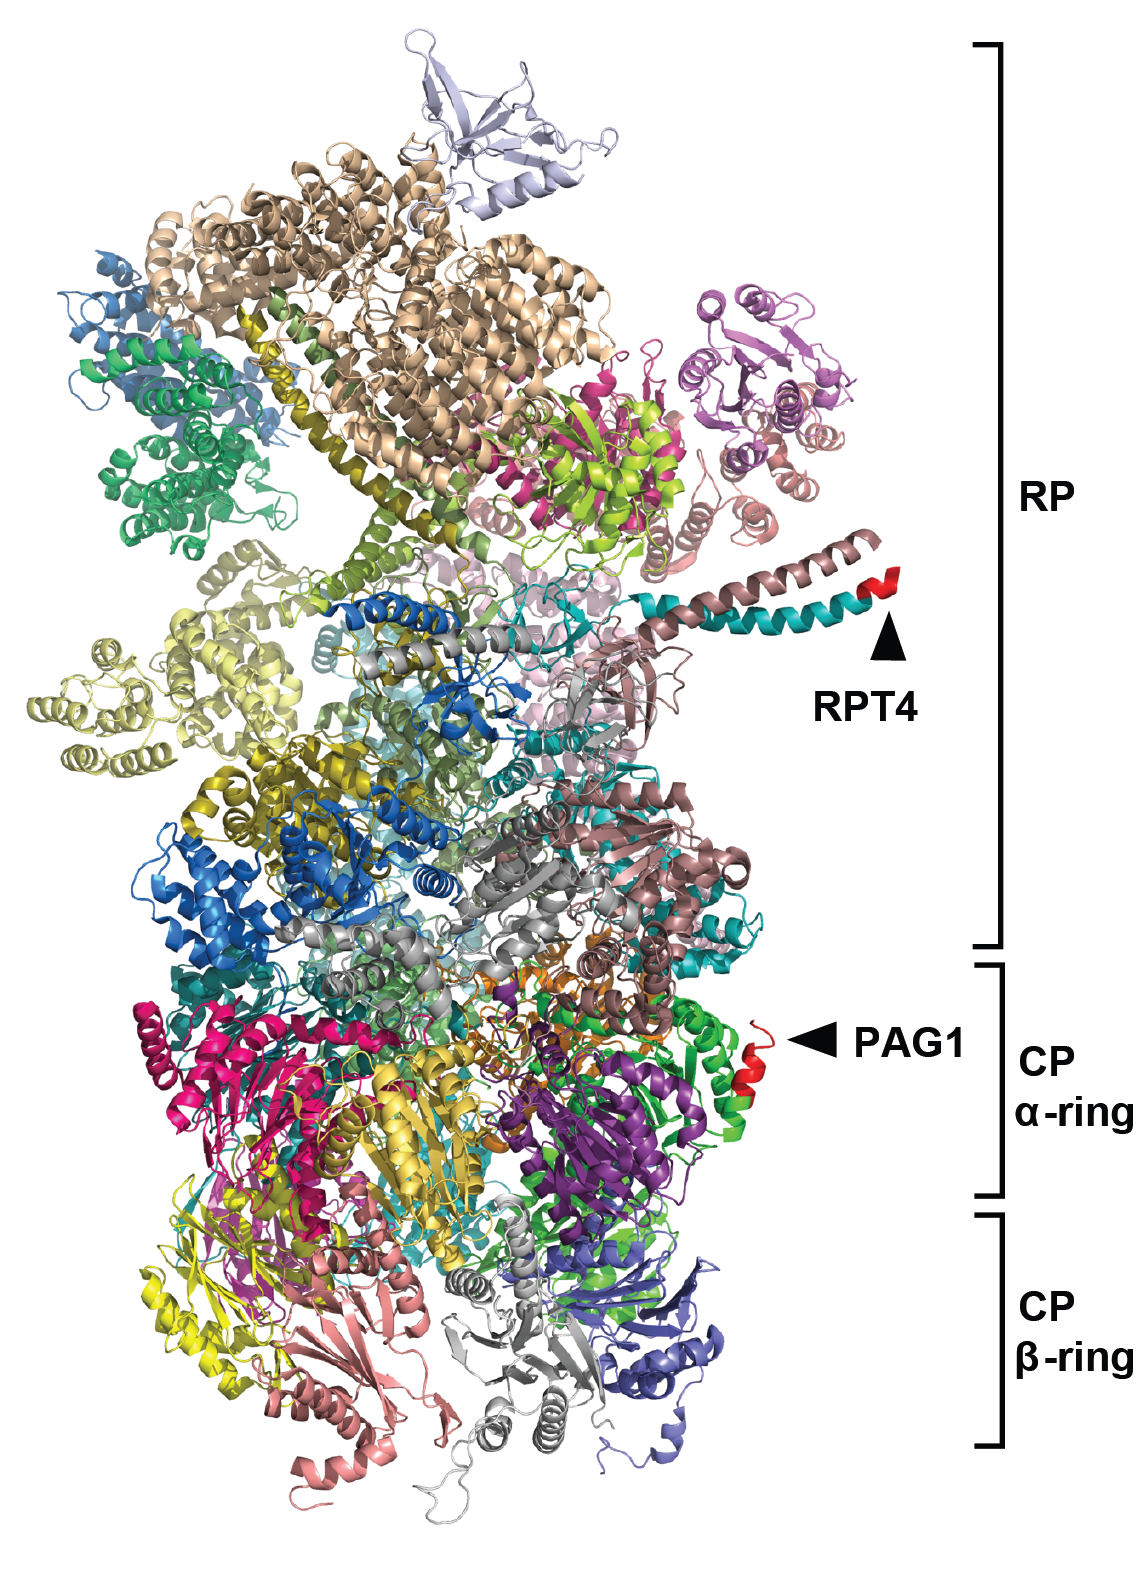
\includegraphics[width=\columnwidth]{intro/taglocations.png}
	\mycaption{Solvent accessible tag locations on the 26S proteasome for both PAG1 and RPT4}
	{A structural model of the 26S proteasome from yeast at sub-atomic resolution modified from PDB ID 4CR2 \citep{beck12}.  The RP subunits, as well as the CP $\alpha$ and $\beta$-rings are shown.  Highlighted in red, and indicated by black arrowheads, are the positions where FLAG affinity tags have been successfully used to enrich for \textit{Arabidopsis} 26S proteasomes.}
	\label{fig:taglocations}
\end{FPfigure}


%ProteasomeAP Leftovers
%\textbf{(C)} Separation of the various proteasome complexes by native PAGE.  26S proteasomes affinity-purified from \textit{PAG1-FLAG} plants as in A were fractioned by native PAGE in the presence of ATP, and the gel was stained for total protein with silver. The migration of the CP alone, the CP-PA200 complex, the RP alone, and 26S proteasomes singly or double capped with RP (26S-1RP and 26S-2RP) are indicated. Additionally, proteasomes can be further subjected to denaturing SDS-PAGE in the second dimension, further confirming the identity of the different species observed by native PAGE. 
\FloatBarrier
\begin{singlespace}
\bibliographystyle{plant_cell_final}
\renewcommand\bibname{Literature Cited}
\bibliography{intro}
\end{singlespace}
